%%%%%%%%%%%%%%%%%%%%%%%%%%%%%%%%%%%%%%%%%
% University Assignment Title Page 
% LaTeX Template
% Version 1.0 (27/12/12)
%
% This template has been downloaded from:
% http://www.LaTeXTemplates.com
%
% Original author:
% WikiBooks (http://en.wikibooks.org/wiki/LaTeX/Title_Creation)
%
% License:
% CC BY-NC-SA 3.0 (http://creativecommons.org/licenses/by-nc-sa/3.0/)
% 
% Instructions for using this template:
% This title page is capable of being compiled as is. This is not useful for 
% including it in another document. To do this, you have two options: 
%
% 1) Copy/paste everything between \begin{document} and \end{document} 
% starting at \begin{titlepage} and paste this into another LaTeX file where you 
% want your title page.
% OR
% 2) Remove everything outside the \begin{titlepage} and \end{titlepage} and 
% move this file to the same directory as the LaTeX file you wish to add it to. 
% Then add \input{./title_page_1.tex} to your LaTeX file where you want your
% title page.
%
%%%%%%%%%%%%%%%%%%%%%%%%%%%%%%%%%%%%%%%%%
%\title{Title page with logo}
%----------------------------------------------------------------------------------------
%	PACKAGES AND OTHER DOCUMENT CONFIGURATIONS
%----------------------------------------------------------------------------------------

\documentclass[12pt]{article} 
 \usepackage[english]{babel}
 \usepackage{apacite}
\usepackage{array,etoolbox}
 \preto\tabular{\setcounter{magicrownumbers}{0}}
 \newcounter{magicrownumbers}
 \usepackage[utf8x]{inputenc}
\usepackage{geometry}
	\geometry{
		a4paper,
		total = {160mm, 245mm},
		left = 30mm,
		top = 30mm
	}
 \usepackage[sort, numbers]{natbib}
  \usepackage{tgbonum}
\usepackage{amsmath}
\usepackage{graphicx}
\graphicspath{{images/}}
\usepackage[colorinlistoftodos]{todonotes}
\usepackage{hyperref}

% \usepackage{amsmath}

\begin{document}

\begin{titlepage}

\newcommand{\HRule}{\rule{\linewidth}{0.5mm}} % Defines a new command for the horizontal lines, change thickness here

\center % Center everything on the page
 
%----------------------------------------------------------------------------------------
%	HEADING SECTIONS
%----------------------------------------------------------------------------------------

\textsc{\LARGE Northeastern University}\\[1.5cm] % Name of your university/college
\textsc{\Large Master's Thesis Proposal}\\[0.5cm] % Major heading such as course name
\textsc{\large CS 7990}\\[0.5cm] % Minor heading such as course title

%----------------------------------------------------------------------------------------
%	TITLE SECTION
%----------------------------------------------------------------------------------------

\HRule \\[0.4cm]
{\Large \bfseries Word-vector Regularization for text classification algorithms}\\[0.4cm] % Title of your document
\HRule \\[1.5cm]
 
%----------------------------------------------------------------------------------------
%	AUTHOR SECTION
%----------------------------------------------------------------------------------------

\begin{minipage}{0.4\textwidth}
\begin{flushleft} \large
\emph{Author:}\\
Ramkishan \textsc{Panthena} % Your name
\end{flushleft}
\end{minipage}
~
\begin{minipage}{0.4\textwidth}
\begin{flushright} \large
\emph{Advisor:} \\
Dr. Virgil \textsc{Pavlu} % Supervisor's Name
\end{flushright}
\end{minipage}\\[.5cm]

\begin{minipage}{0.82\textwidth}
\begin{flushright} \large
\emph{Official Reader:} \\
Dr. Byron \textsc{Wallace} % Reader's Name
\end{flushright}
\end{minipage}\\[2cm]

% If you don't want a supervisor, uncomment the two lines below and remove the section above
%\Large \emph{Author:}\\
%John \textsc{Smith}\\[3cm] % Your name

%----------------------------------------------------------------------------------------
%	DATE SECTION
%----------------------------------------------------------------------------------------

{\large \today}\\[2cm] % Date, change the \today to a set date if you want to be precise

%----------------------------------------------------------------------------------------
%	LOGO SECTION
%----------------------------------------------------------------------------------------


\includegraphics[width=4cm, height=4cm]{logo.jpg}\\[1cm] % Include a department/university logo - this will require the graphicx package
 
%----------------------------------------------------------------------------------------

%\vfill % Fill the rest of the page with whitespace

\end{titlepage}
% \begin{abstract}
A simple and efficient baseline for text classification is to represent sentences as bag-of-words (BoW) and train a linear classifier. The bag-of-words model is simple to implement and offers flexibility for customization by providing different scoring techniques for user specific text data. In many problem domains, these linear classifiers are preferred over more complex models like CNN, LSTM because of their efficiency, robustness and interpretability.

However, a large vocabulary can cause extremely sparse representations which are harder to model, where the challenge is for models to harness very little information in such a large representational space. Also, these classification problems are categorized by large number of classes and highly imbalanced distribution of data across these classes. In such cases, the traditional linear classifiers would treat each word separately and assign them different coefficients based on the frequency in which they occur in the train set. This would result in lower test accuracy when it comes across instances where a word which was occurring less frequently in the train set, occurs more often in the test set.

Our thesis aims to solve this problem by constraining weights of rare features by similar, more frequent ones, using semantic similarity. This would enforce similar words to have similar weights thereby improving model performance. Thus, based on how similar two features are, our proposed model can improve the feature importance of a sparse word by increasing its regression co-efficient, thereby improving the test accuracy in the above mentioned scenario.

\end{abstract}

\section{Introduction}

The goal of text classification is to classify text documents into one or more classes according to their content. For this purpose, a document must be transformed into a representation which is suitable for the learning algorithm and the classification task. Representing documents as bag-of-words is a commonly used method in document classification where the frequency of occurrence of each word is used as a feature for training a classifier. However, one should note that when using this representation, some document information is lost as the model disregards grammar and word ordering.

\subsection{Problem Statement}

Although the bag-of-words model is widely used and performs exceptionally well in most text classification problems, it contains several limitations. As per Zipf's law \cite{li1992random}, given a large sample of words used, the frequency of any word is inversely proportional to its rank in the frequency table. So, word number n has a frequency proportional to 1/n. Thus, a large vocabulary can cause extremely sparse representations. 

The classification accuracy we observe on the test set largely depends on the quality of training sets we have used to build our models. That is, if the training information is sparse, then we can expect the category model to be a poor representation of a category thereby leading to poor classification accuracy. Words that occur rarely do not give a learning algorithm enough information to determine its influence on classification correctly.

Thus, in such a case any linear classifier like logistic regression, naive bayes, linear SVM would treat each word independently and assign them different coefficients based on the impact of the individual word on the response variable. As the training data for rare words would be sparse, their coefficients would be near 0 implying that the impact of these features is small. This may not be the case as these rare words might be misrepresented due to sparse data. Our model tries to solve this problem by using a word-vector regularizer that assigns similar coefficients to words which are used in a similar context, thereby boosting the effect of similar but rare features on the final prediction.

We use logistic regression for binary text classification on a bag-of-words model. Let $\theta^{(i)}$ be the regression coefficients of word$_{i}$ which determines the association between each feature value (word occurrence in document) and what the target we are trying to predict.

\noindent The cost function for logistic regression would be given as:

\begin{equation}\label{lr_cost_fn_eq}
Cost(h_{(\theta)}(x), y) = 
\begin{cases}
-log(h_{(\theta)}(x)), $\qquad if y=1$
\\
-log(1-h_{(\theta)}(x)), $ if y=0$
\end{cases}
\end{equation}\\

In general, the features with larger coefficients are more important because they make a significant contribution in predicting the correct class. However if a word$_{k}$ is rare, its corresponding regression coefficient ($\theta^{(k)}$) could be very small or very large (minimizing the loss) due to lack of evidence in the training set; which is not useful for predictions. Our plan here is to constrain such coefficients by the word semantic similarity with other more frequent terms, thus simulating a higher occurence and prohibiting extreme behavior. This also helps with non-frequent synonym words in making their coefficients more uniform. \\

\noindent \textbf{Example:} In order to get a better understanding, consider a classification problem where we are trying to identify whether a document is talking about animals or not. For this example, let's say we only have five features. The bag-of-words representation using term frequencies for 5 different documents would look like:

\begin{table}[htbp]
\centering
\begin{tabular}{l|lllll}
 & dog & \multicolumn{1}{c}{football} & \multicolumn{1}{c}{canine} & movies & cat \\\hline
D1 & 3 & 0 & 0 & 0 & 4 \\
D2 & 0 & 0 & 0 & 6 & 0 \\
D3 & 5 & 0 & 1 & 0 & 6 \\
D4 & 0 & 8 & 0 & 0 & 0 \\
D5 & 0 & 7 & 0 & 4 & 0
\end{tabular}
\caption{Toy dataset}
\end{table}

From the above example, we can see that the word ‘canine’ occurs only once in one of the document. If we train a linear classifier on the above dataset, then ‘canine’ would have a very low feature importance due to its sparse representation. When we test this classifier on a document where ‘canine’ is more densely represented as compared to ‘dog’ or ‘cat’, then that document would get misclassified as “not talking about animals”. 

In contrast, since our model would assign similar weights to similar words and considering ‘dog’ and ‘canine’ are synonyms, our model would assign a higher feature importance to ‘canine’, thereby increasing the probability of making a correct prediction on a new document where ‘canine’ is more densely represented as compared to the train data.

\subsection{Related work}
A number of approaches have been proposed to increase the classification accuracy on the bag-of-words model.

To aggressively reduce the dimensionality of models, Joachims \cite{joachims1996probabilistic} (1996), Yang and Pedersen\cite{yang1997comparative} (1997) suggested pruning of infrequent words. Mansuy and Hilder \cite{mansuy2006characterization} (2006) recommended removing of stop words and part-of-speech tags. Porter \cite{porter1980algorithm} (1980) proposed removal of suffixes from words. However, Joachims \cite{joachims1996probabilistic} test results revealed that the performance of the system is higher when more words are used as features, with the highest performance achieved using the largest feature set. Any approach that limited the number of words to the most important ones was likely to reduce the classification accuracy as these pruned words lose their ability to contribute to the classification of text. Quinlan \cite{quinlan2014c4} (1993) suggested choosing words which have high mutual information with the target concept. However, picking words with high mutual information had relatively poor performance due to its bias towards favoring rare terms, and its sensitivity to probability estimation errors.

In an attempt to address the issue of related concepts in text classification, many researchers have incorporated features using dictionaries and encyclopedias. Mavroeidis et. al \cite{mavroeidis2005word} (2005) proposed to extend the traditional bag of words representation by incorporating syntactic and semantic relationships among words using a Word Sense Disambiguation approach. Wang and Domeniconi \cite{wang2008building} (2008) explored a similar approach by embedding background knowledge derived from Wikipedia to enrich the representation of documents. Although empirical results have shown improvements in some cases, the applicability of using dictionaries to improve classification accuracy is limited. Ontology is manually built, and the coverage is far too restricted. Recently, Heal et. al \cite{heap2017word} (2017) introduced a method for enriching the bag-of-words model by complementing rare term information with related terms from Word Vector models. However, it was revealed that these methods achieved significantly better results only when the training sets were small. There wasn't enough evidence of achieving better results on large datasets.

In addition to incorporating related concepts to improve classification performance, other approaches have also been proposed. One of these approaches considers using part-of-speech tags associated with words contained in a document (Scott and Matwin \cite{scott1998text} 1998), (Jensen and Martinez \cite{jensen2000improving} 2000). Since words can have multiple meanings depending upon how and where they are used in a sentence, the part-of-speech may be relevant to text classification. However, a different paper from Mansuy \cite{mansuy2006characterization} revealed that there was no significant difference between the accuracy of the classifiers whether part-of-speech tags are utilized or not.

To deal with overfitting, different regularization techniques have also been proposed. Regularization adds a penalty on the different parameters of the model to reduce the freedom of the model. Hence, the model will be less likely to fit the noise and improve its generalization abilities. The Lasso regularization acts as a way of feature selection by shrinking some parameters to zero, whereas the Ridge regularization will force the parameters to be relatively small but are not cut to zero.
\newpage
\section{Word-Vectors}

Word vectors represent a significant leap forward in advancing our ability to analyze relationships across words, sentences, and documents. In doing so, they advance technology by providing machines with much more information about words than has previously been possible using traditional representations of words. It is word vectors that make technologies such as Machine translation, Sentiment analysis, Speech recognition, Question Answering possible.\\

\noindent This chapter will explain the following:
\begin{itemize}
\item{Need for word-embeddings}
\item{History of word-embeddings}
\item{Word-vector training}
\item{Semantic Relationship and similarity}
\item{Word Pairs and Phrases}
\item{Applications of word embeddings}
\item{Current advances in word-embeddings}
\end{itemize}

\subsection{Need for word-embedding}

Traditional NLP systems treated words as atomic units, such as one-hot encoding and bag-of-words models. These methods used dummy variables to represent the presence or absence of a word in an sentence. For the one-hot encoding, each word is represented by a one-hot vector - a sparse vector in the size of the vocabulary, with 1 representing the presence of a word and 0 representing its absence. The bag-of-words feature vector considers the word occurrence as feature value which is normalized using term frequency and inverse-document frequency to increase the importance of rare words and reduce the importance of very frequent but less important words like stop words.

This choice of word-representation is simple, robust and can act as a good baseline model which can be coded using a few lines of code. It also works very well when your dataset is small and the context is domain specific. However these models do not preserve the semantic relationship between words and hence lose important linguistic patterns such as word-order and synonyms. Ex. "This is good" and "Is this good" have the same feature representation. They are also difficult to model highly sparse data. Thus, simple scaling up of basic techniques will not result in any significant progress, and we have to focus on more advanced techniques.

\newpage
\subsection{History of word-embeddings}

The technique of representing words as vectors has roots in the 1960s with the development of vector space models for information retrieval. Reducing the number of dimensions using singular value decompostitoin led to the introduction of latent semantic analysis in the late 1980s. In 2001, Bengio et al. \cite{bengio2003neural} published a paper to tackle language modeling and it was the initial idea of word-embedding. At that time, they named this process as "learning a distributed representaion for words".

In 2008, Ronan and Jason \cite{collobert2008unified} introduced a concept of pre-trained model and showed its amazing approach for solving NLP problems. In 2013, a team at Google led by Tomas Mikolov created word2vec \cite{mikolov2013efficient}, a word-embedding toolkit which can train vector space models faster than the previous approaches. Later on, gensim provided an amazing wrapper so that adopt different pre-trained word-embedding models which include Word2Vec (by Google), GloVe \cite{pennington2014glove} (by Stanford), fastText (by Facebook).

\subsection{Word-vector training}

Training a word2vec model is similar to an autoencoder. We use a simple neural network with a single hideen layer to perform a certain task, but then we're not going to use it for the task we trained it for. Instead, the goal is to just learn the weights of the hidden layer that are actually the word-vectors that we're trying to learn.

Training the model is done in one of two ways, either using the context to predict a target word (known as continuous bag of words or CBOW) or using a word to predict a target context, which is called skip-gram. According to Mikolov, the skip-gram model works well with small amount of training data and represents well even rare words or phrases. The CBOW is several times faster to train than the skip-gram and shows slightly better accuracy for the frequent words. Let us first look at the skip gram model.

We're going to train the neural network to do the following: Given a specific word in the middle of a sentence (the input word), look at the nearby words and pick one at random. The network is going to predict the probability for every word in the vocabulary of being the nearby word that we choose. The nearby word is actually a window size parameter to the algorithm. A typical window size might be 5.

The output probabilities indicate how likely is it to find each word near our input word. For example, the input word "Soviet" will have higher probabilities for words like "Union" and "Russia" than for unrelated words like "watermelon" and "kangaroo". The neural network will be trained by feeding it word pairs from the train data. The below example shows some of the training samples. The word highlighted in blue is the input word.

\begin{figure}[htbp]
\centering
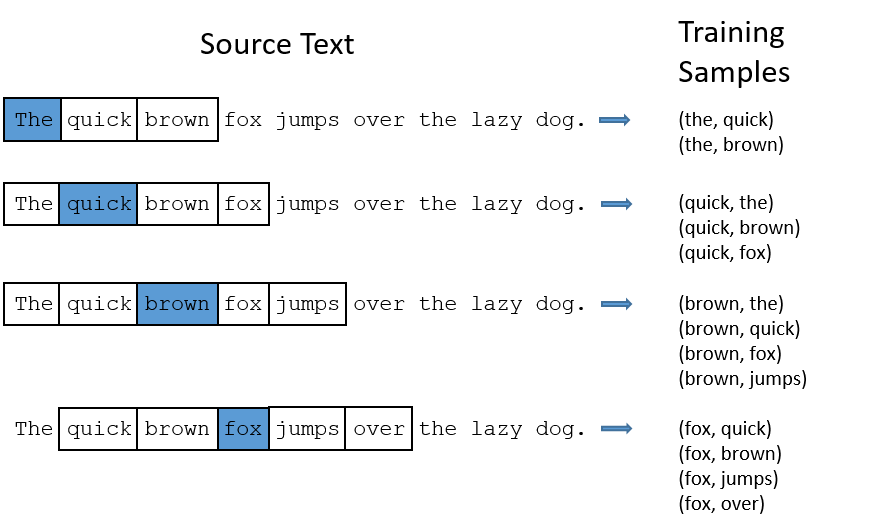
\includegraphics[width=16cm, height=10cm]{images/training_data.png}\\
\centering
\caption{Training samples for skip-gram model having a window size of 2.}
\label{fig:foo}
\end{figure}

\newpage
\subsubsection{Model details}

The words cannot be fed to the neural network as a text string. To do this, we represent the words as a one-hot vector. If we have a vocabulary of 10,000 unique words, then the one-hot vector will have 10,000 components (one for every word in the vocabulary) and we'll place a 1 in the position corresponding to the word and 0 in all other positions. The output of the network is also a single vector with 10,000 components containing the probability that a randomly selected nearby word is that vocabulary word. Thus, the output vector will actually be a probability distribution and not a one-hot vector.

If we want to learn our word-vectors with 300 features, the hidden layer would be represented by a weight matrix with 10,000 rows and 300 columns and the end goal is just to learn the hidden layer weight. The output layer is trained using a softmax regression classifier. The network diagram for both the skip-gram and continuous bag of words models can be seen in the next page.

\begin{figure}[htbp]
\centering
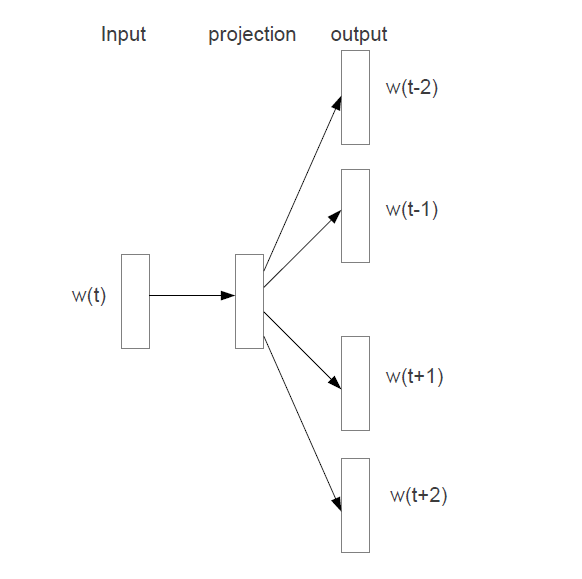
\includegraphics[width=16cm, height=10cm]{images/skip-gram.PNG}\\
\centering
\caption{Skip-gram model: Predicts the surrounding words given the current word.}
\label{fig:foo}
\end{figure}

\begin{figure}[htbp]
\centering
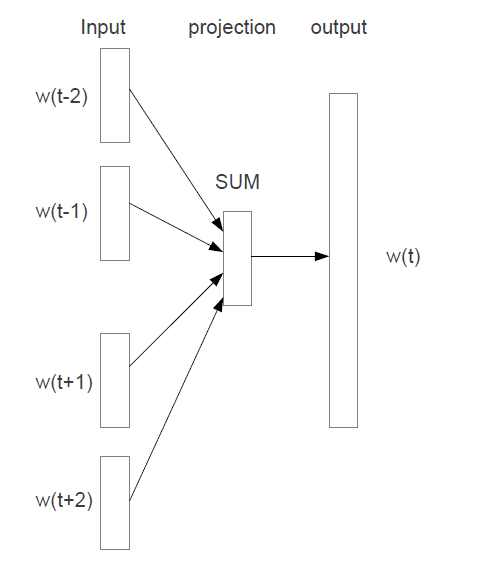
\includegraphics[width=16cm, height=10cm]{images/CBOW.PNG}\\
\centering
\caption{Continuous Bag of words model: Predicts the current word given the context.}
\label{fig:foo}
\end{figure}

\subsubsection{Improvements to the model}

From the previous example, we've seen that for word-vectors with 300 components and 10,000 vocabulary size, both the hidden and output layers will have the weight matrix of size 300 x 10,000 = 3 million weights each. Running gradient descent on a neural network that large is going to be slow. To address this issue, the word2vec authors addressed this issue in their paper with the following two innovations:

\begin{itemize}
\item{subsampling frequent words to decrease the number of training examples}
\item{modifying the optimization objective through "Negative sampling" which causes each training sample to update only a small percentage of model's weights.}\\
\end{itemize}
\noindent\textbf{Subsampling Frequent words:}\\

In the previous example of the sentence, "The quick brown fox jumps over the lazy dog.", we've seen two common problems. Firstly, word pairs like (fox, the) doesn't tell us much about the meaning of "fox" as "the" appears in the context of almost every word. Secondly there are many samples of "the" than needed to learn a good vector for it. To remediate this, word2vec implements a subsampling scheme that subsamples some of the words from the training data based on its frequency.\\

\noindent\textbf{Negative Sampling:}\\

Instead of every training sample tweaking all the weights of the neural network, we can modify only a small percentage of weights, rather than all of them. With negative \cite{goldberg2014word2vec}, we are going to randomly select a small number of negative weights to update along with updating all the positive weights. The negative samples are selected using a unigram distribution, where frequent words are more likely to be selected as negative samples. Thus the probability of picking the word as part of a negative sample to update will depend on the number of times the word appears in the corpus divided by the total number of words in the corpus. This is expressed by the following equation:

\begin{equation}
P(w_{i}) = \frac{f(w_{i})}{\sum_{j=0}^{n}f(w_{j})}
\end{equation}

The word vector space implicitly encodes many regularities among words. The resulting distributed representation of words contain a lot of syntactic and semantic information which we will see in the next section.

\subsection{Semantic Relationship and Similarity}

Word vectors represent words as a vector of real valued numbers where each point captures a dimension of the word's meaning. Thus, if two different words have very similar "contexts" i.e., what words are likely to appear around them, then the model needs to output very similar results for these two words. And one way for the network to output similar context predictions for these two words is if the word-vectors are similar. So, if two words have similar contexts, then the network will eventually learn similar word vectors for these two words. This means that words such as "engine" and "transmission" should have similar word vectors to the word "car", whereas the word "pineapple" should be quite distant. This can also handle stemming for you - the network will likely learn similar word-vectors for words like "man" and "men" because these should have similar contexts.

\newpage

\begin{figure}[htbp]
\centering
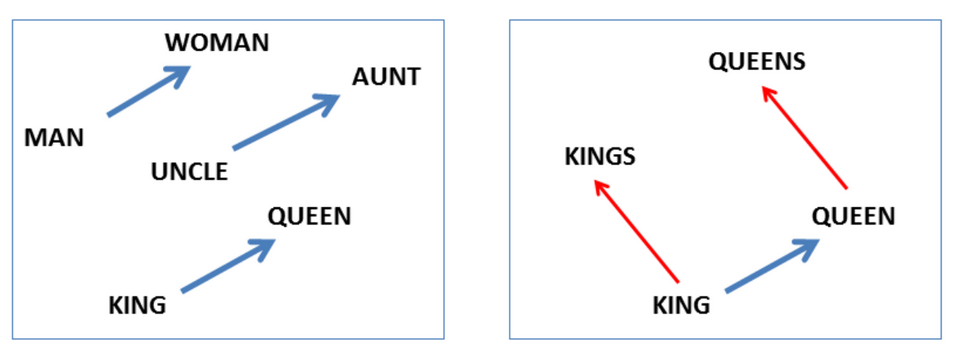
\includegraphics[width=12cm, height=6cm]{images/wv-similarities.PNG}
\centering
\caption{The word vector space encodes many regularities among words.}
\label{fig:foo}
\end{figure}

\noindent \textbf{Analogies:}\\

The famous examples that show incredible properties of embeddings is the concept of analogies. We can add and subtract word embeddings and arrive at interesting results. The most famous example is the formula:
\begin{itemize}
\item{"king" - "man" + "woman" = "queen"}
\end{itemize}
In other words, we can subtract one meaning from the word vector for king (i.e. maleness), add another meaning (femaleness), and show that this new word vector maps closely to the word vector for queen.

\begin{figure}[htbp]
\centering
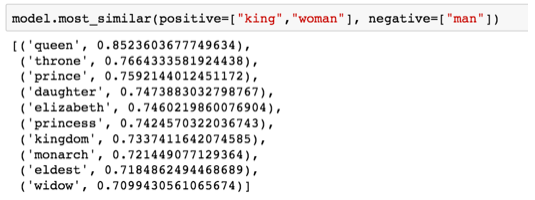
\includegraphics[width=16cm, height=8cm]{images/king-man+woman-gensim.png}\\
\centering
\caption{The image shows that we can add and subtract word vectors and it would find the most similar words to the resulting vector.}
\label{fig:foo}
\end{figure}

\newpage
\subsection{Word Pairs and Phrases}

The current implementation of word vectors is limited to its unigram natural behavior. It does not embed bigrams like "American Airlines" as its whole. In some cases, a word pair like "Boston Globe" (a newspaper) has a much different meaning than the individual words "Boston" and "Globe". So it makes sense to treat "Boston Globe" as a single term whenever it occurs when its own word vector representation.

However, the addition of phrases to the model will exponentially increase the vocabulary size. The word2vec team have built a tool that counts the number of times each combination of two words appears in the training text, and use it in an equation to determine which word combinations turn into phrases \cite{mikolov2013distributed}. The equation is designed to make phrases out of words which occur together often relative to the number of individual occurrences. It also favors phrases made of infrequent words in order to avoid making phrases out of common words like "and the" or "this is".

The same word2vec idea can be extended to sentences and complete documents where instead of learning feature representation for words, you learn it for sentences or documents. The applications of these models could depend on the task at hand. A word2vec model can effectively capture semantic relationship between words and hence it can be used to calculate word similarities or fed as features to various NLP tasks such as sentiment analysis, LSTMs etc. However words can only capture so much, there are times when you need relationships between sentences and documents and not just words. For example, if you are trying to figure out if two documents are duplicates of each other.

\subsection{Applications of word embeddings}

Word embeddings are used in almost all NLP tasks these days:

\begin{itemize}
\item In conjunction with modelling techniques such as deep neural networks, word embeddings have massively improved text classification accuracy in many domains including customer service, spam detection, document classification etc.

\item Word vectors are also used to build language models which predict the next most probable words given the current word. This is learnt through a deep lstm network called Seq2Seq learning. Few applications of these language models are Gmail autoreply and Google search.

\item Seq2Seq models with attention gives state of the art accuracy for machine translation.
\end{itemize}

\begin{figure}[htbp]
\centering
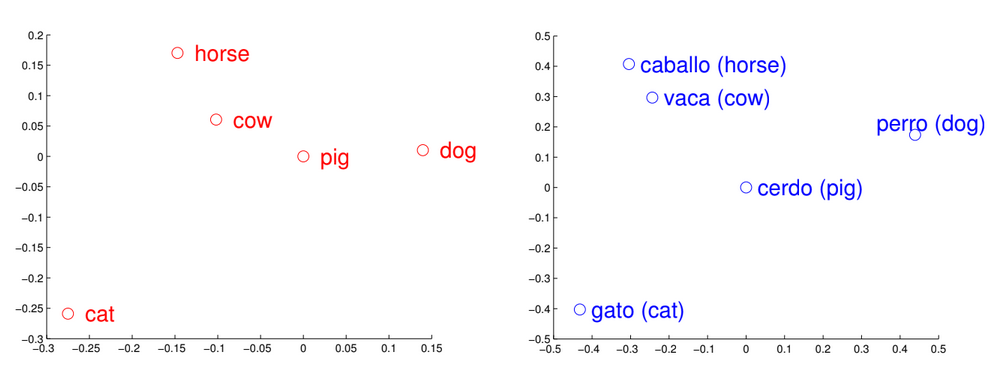
\includegraphics[width=16cm, height=8cm]{images/machine-translation.PNG}\\
\centering
\caption{Machine Translation - English to Spanish. Example showing word vectors having similar structure when trained on comparable corpora}
\label{fig:foo}
\end{figure}

\newpage
\subsection{Current advances in word embeddings}

Though pre-trained word embeddings have been very influential, they have a major limitation - they presume that a word's meaning is stable across sentences. However this approach to word representation does not address polysemy, or the co-existence of many possible meanings for a given word or phrase. There can be cases where there are major differences in meaning for a single word: e.g. get (a verb for obtaining) and get (an animal's offspring); or bank (a financial institution) and bank (someone to rely on). Also traditional word vectors are a single layer of weights, a shallow representation. Such word vectors fail to capture higher-level information that might be even more useful. Recent advances in NLP go from just initializing the first layer of the model to pre-training the entire model with hierarchical representations to make the model capable of performing diverse range of tasks including question answering, natural language inference etc.\\

\noindent \textbf{Embeddings from Language Models (ELMo)}\\

The motivation for ELMo \cite{peters2018deep} is that word embeddings should incorporate both word-level characteristics as well as contextual semantics. So instead of taking just the final layer of deep bi-LSTM language model as the word representation, ELMo embeddings are a function of all internal layers of bi-LSTM. The intutition is that higher level states of the bi-LSTM capture context, while lower level captures syntax. Thus, instead of using a fixed embedding for each word, ELMo looks at the entire sentence before assigning each word an embedding thus generating different embeddings for each of its occurence.

\newpage
\noindent \textbf{Open AI GPT (Generative Pre-training Transformer)}\\

Open AI GPT \cite{radford2018improving} is similar to ELMo, with a few differences. Firstly while ELMo uses Bi-LSTMs, GPT is a multi-layer encoder-decoder model with attention mechanism. Secondly while ELMo feeds embeddings into models for customized tasks, GPT fine tunes the same base model for all tasks.

However, one drawback of the GPT is its uni-directional nature - the model is only trained to predict the future left-to-right context.\\

\noindent \textbf{Bidirectional Encoder Representations from Transformers (BERT)}\\

BERT \cite{devlin2018bert} is a direct descendent to GPT — train a large language model on free text and then fine-tune on specific tasks without customized network architectures. Compared to GPT, the largest difference and improvement of BERT is to make training bi-directional. The model learns to predict both context on the left and right. The model architecture of BERT is a multi-layer bi-directional Transformer encoder.
\section{Proposed Method}

In this method, we propose to enhance the bag-of-words model for text classification by adding additional features to the vanilla logistic regression model. These new features will act as a regularizer which would assign similar coefficients to words used in similar context.

\begin{figure}
\centering
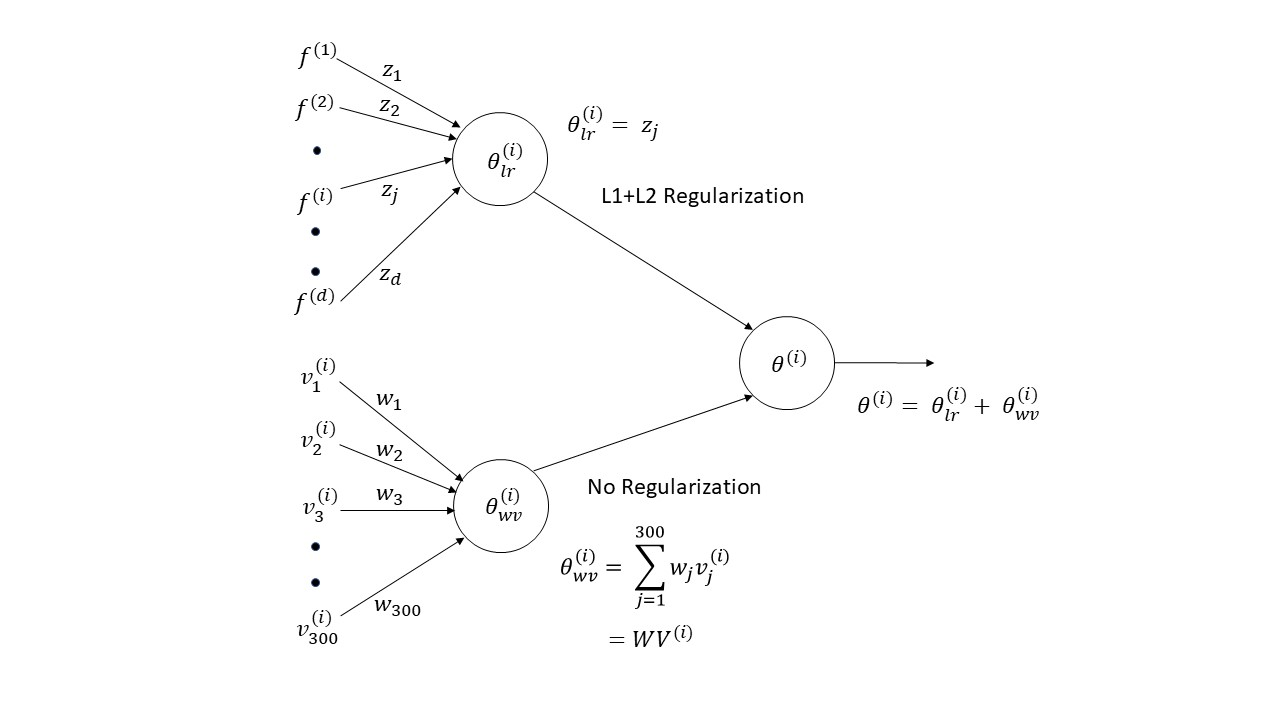
\includegraphics[width=16cm, height=10cm]{images/Fig3.jpg}\\
\centering
\caption{Network diagram to learn $\theta^{(i)}$ from word$_{i}$ representation f(v$^{(i)}$)}
\label{fig:foo}
\end{figure}

The problem we are trying to solve can be formulated as follows: Given a set of m documents with n features, the documents would be represented by matrix X $\in$ R$^{m x n}$. We want to find the coefficients that predict the output Y from the documents X and we want to build a model where the coefficients ($\theta^{(i)}$) are a sum of the weights learnt through logistic regression and a function of its word$_{i}$ representation ($v^{(i)}$), i.e.,

\begin{equation}\label{lb1}
\theta^{(i)} = \theta_{lr}^{(i)} + \theta_{wv}^{(i)}
\end{equation}

These new weights $\theta_{wv}^{(i)}$ would act as a regularization constraint so that similar word representations would have similar coefficients, which satisfies a continuity condition:

\begin{equation}
|f(v^{(1)}) - f(v^{(2)}))|\ \leq\ sim(v^{(1)}, v^{(2)})
\end{equation}

where, $sim$ dictates the similarity between words $v^{(1)}$ and $v^{(2)}$ and $ f(v^{(1)}), f(v^{(2)})$ are coefficients of their respective words as per (\ref{lb1})

% $\quad\qquad\ \epsilon $ is the smallest constant satisfying the equation (Lipschitz constant)\\

Since words used in similar context will have similar word-vectors and by making the regression co-efficient of a word to be a function of its word-vector representation, we can regularize the regression coefficients of two similar words to have similar values. So, if one word occurs more frequently and has higher regression co-efficient, the other word even if it is very rare would be considered an important feature and would have a higher regression co-efficient. This would improve the classification performance in cases where these rare words occur more frequently in the test set.\\

% Our goal is to regularize the text classifier coefficients using word-vectors. However, for the thesis our objective is to learn the function $f(v^{(i)})$ and use it to regularize regression on text. \\

\noindent Fig. 1 is a network diagram showing how the coefficients ($\theta_{i}$) would be obtained for a word$_{i}$ representation using both the above mentioned method.\\\\\\\\

\noindent We initially explore learning $\theta_{wv}^{(i)}$ through regression:\\

%\begin{itemize}
%\item regression
%\item 2-layer neural network
%\item boosting trees
%\end{itemize}


%%%%%%%%%%%%%%%%%%%%%%%%%%%%%%%%%%
\noindent\textbf{Learning $\theta_{wv}^{(i)}$ through Regression}: We determine if we can learn the coefficients $\theta_{wv}^{(i)}$ from the word representation of the features using a linear regressor, i.e., 

\begin{equation}
\theta_{wv}^{(i)} = w_{1}v_{1}^{(i)} + w_{2}v_{2}^{(i)} + ... + w_{d}v_{d}^{(i)} = \sum_{d=1}^{D} w_{d}^{(i)}v_{d}^{(i)}
\end{equation}

where, $w = (w_{1}, w_{2}, ..., w_{d})$ are the parameters of the regression function. 

$\quad\qquad\  v= (v_{1}, v_{2}, ..., v_{d})$ are d-dimensional word-representations of word $i$\\

\noindent These new weights which have been regularized through word-vectors will act as additional features to the free weights learnt through the vanilla logistic regression model. Thus the probability that class variable $y_{j}=1, j=1,2,...m$ can be modelled as follows:

\begin{equation}
P(y_{j} = 1 | x_{j}; \theta, w) = h_{(\theta| w)}(x_{j}) = \frac{1}{1+e^{-\theta^{T}x_{(j)}}}
\end{equation}

where, $\theta^{(i)} = \theta_{lr}^{(i)} + \theta_{wv}^{(i)}$ are the parameters of the function for feature (i)\\

\noindent Within the class of linear functions, our task shall be to find the best parameters $w$ that minimize the error function such that,

\begin{equation}\label{cost_fn_eq}
Cost(h_{(\theta| w)}(x), y) = 
\begin{cases}
-log(h_{(\theta| w)}(x)), $\qquad if y=1$
\\
-log(1-h_{(\theta| w)}(x)), $ if y=0$
\end{cases}
\end{equation}\\
%%%%%%%%%%%%%%%%%%%%%%%%%%%%%%%%%%

% \noindent\textbf{Learning f as 2-layer neural network}: If there is a non-linear relationship between the coefficients and word representations, we can learn them through a multi-layer neural network. We start with a 2-layer neural network having one hidden layer and one output layer. The hidden layer requires the d-dimensional word$_{i}$ representations as input and outputs an activation value.\\\\ Let $a^{[1](i)} = (a^{[1](i)}_{1},a^{[1](i)}_{2},a^{[1](i)}_{3}..)$ be the activation of the neurons in the hidden layer, and $a^{[2](i)}$ be the activation of the neurons in the output layer.\\

% \noindent where, a = g(z), where g is some activation function (like sigmoid, relu, tanh)

% \quad\quad z = Wx + b, where x are the features from the input layer

% \quad\quad a$^{[l]}_{k}$ denotes the activation of the $k^{th}$ unit in layer $l$

% \quad\quad $x^{(i)}$ with parenthesis refers to the i$^{th}$ word

% \quad\quad a$^{[1]}$ is the concatenation of all first layer activations\\

% \noindent For a 2-layer neural network, we would have the following parameters:

% \begin{alignat}{2}
% z^{[1](i)} & = W^{[1]}V^{(i)} + b^{[1]}\\
% a^{[1](i)} & = g(z^{[1](i)})\\
% z^{[2](i)} & = W^{[2]}a^{[1](i)} + b^{[2]}\\
% \theta^{(i)} & = a^{[2](i)} = g(z^{[2]})
% \end{alignat}

% \noindent We can then train a neural network model to learn the coefficients ($\theta^{(i)}$) which would help minimize the cost function in (\ref{cost_fn_eq})

% \section{Implementation}

\subsection{Obtain word-vectors}

Out of the successful deep learning models used for word-embeddings, two of the most popular ones are Word2Vec \cite{le2014distributed} and Global Vectors \cite{pennington2014glove}. For our research, we will be using Google's Word2Vec which has pre-trained word-vectors with 300 dimensions trained using over 100 billion words. 

Also it has been seen that a smaller domain specific Word Vector model is modelled better than a general model trained over a much larger corpus of text. Thus Google's pre-trained Word Vector model which was trained over three million unique words and phrases will be retrained on the training data to generate domain specific Word Vectors.

\subsection{Train new model}

Once the features have been extracted using the bag-of-words model and their corresponding word-vectors obtained, we can train a neural network model based on the cost function in (\ref{cost_fn_eq})\\

\noindent Below is the link to its source code on GitHub. It will be made publicly available upon thesis completion:

\noindent \url{https://github.com/RamkishanPanthena/Master-s-Thesis}
\newpage
\section{Initial models tested}

\subsection{Document embedding by averaging word-vectors}

We initially tried a basic scenario where documents are represented by a fixed length vector which can then be used for classification even though each document can be of a different length.

One of the common techniques to generate new embeddings to documents is by using an existing pre-trained word embeddings by averaging the word vectors to create a single fixed size embedding vector.

\begin{figure}[htbp]
\centering
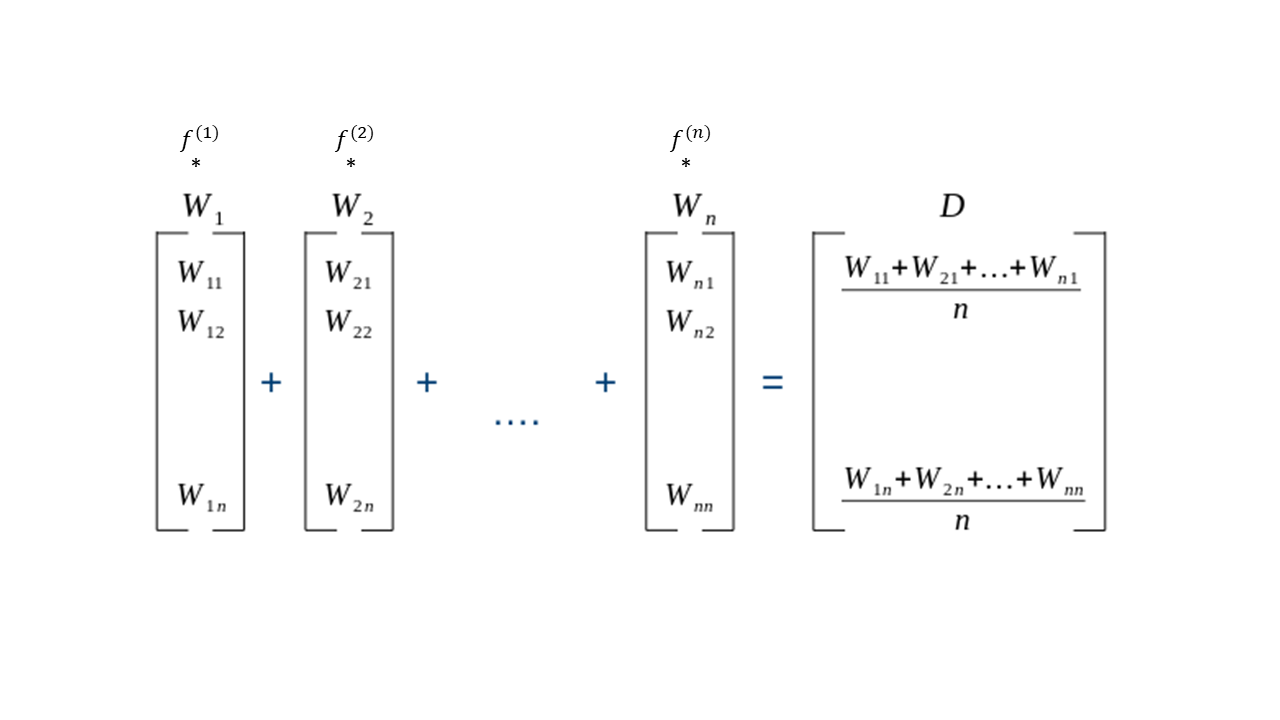
\includegraphics[width=16cm, height=8cm]{images/average-vectors.png}\\
\centering
\caption{Average word-vectors}
\label{fig:foo}
\end{figure}

\subsubsection{Steps to compute fixed embedding vector}

\begin{itemize}
\item {First we import a word vector model that either has been pre-trained by Google or retrained on the training data to obtain domain specific word vectors.}
\item {Then we iterate over the entire corpus and generate a mean vector for each document.}
\end{itemize}
Once we obtain the mean vector for all the documents, we train a vanilla logistic regression model using the thus generated fixed embedding feature matrix.

\begin{figure}[htbp]
\centering
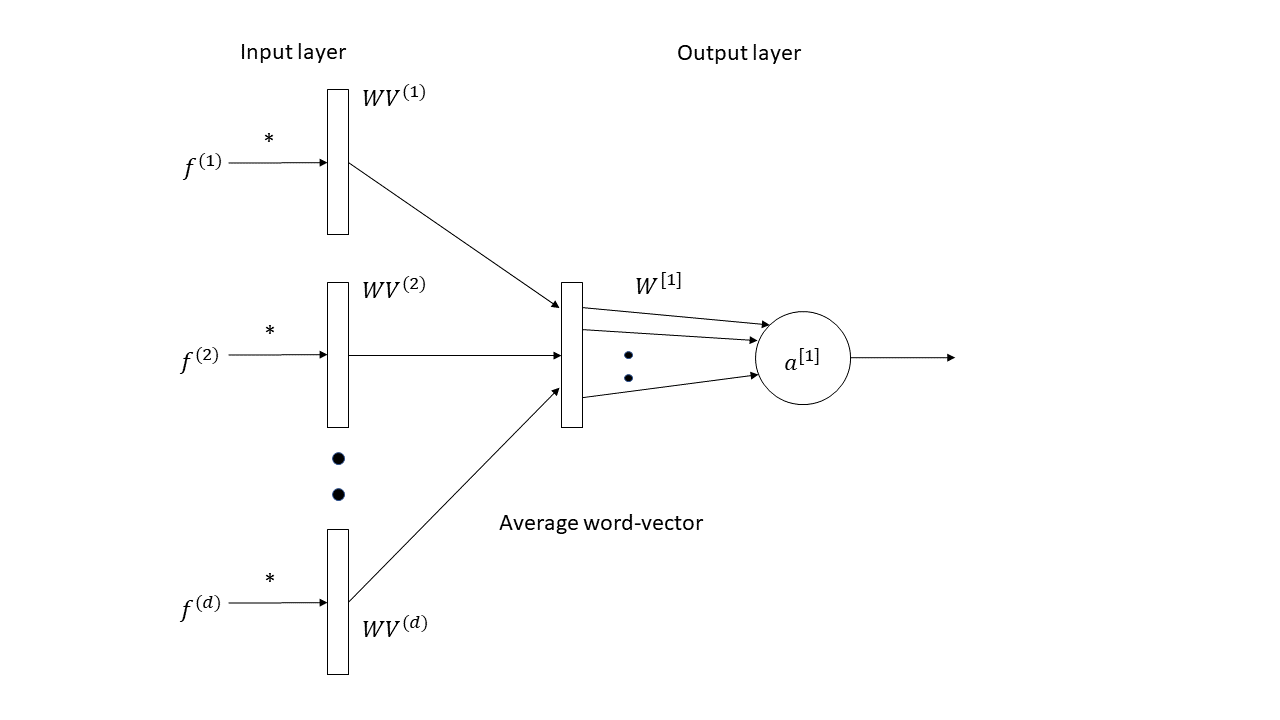
\includegraphics[width=16cm, height=8cm]{images/average-vectors2.png}\\
\centering
\caption{Average word-vectors model}
\label{fig:foo}
\end{figure}

\newpage
\subsection{Initial word-vector model}

\begin{figure}[htbp]
\centering
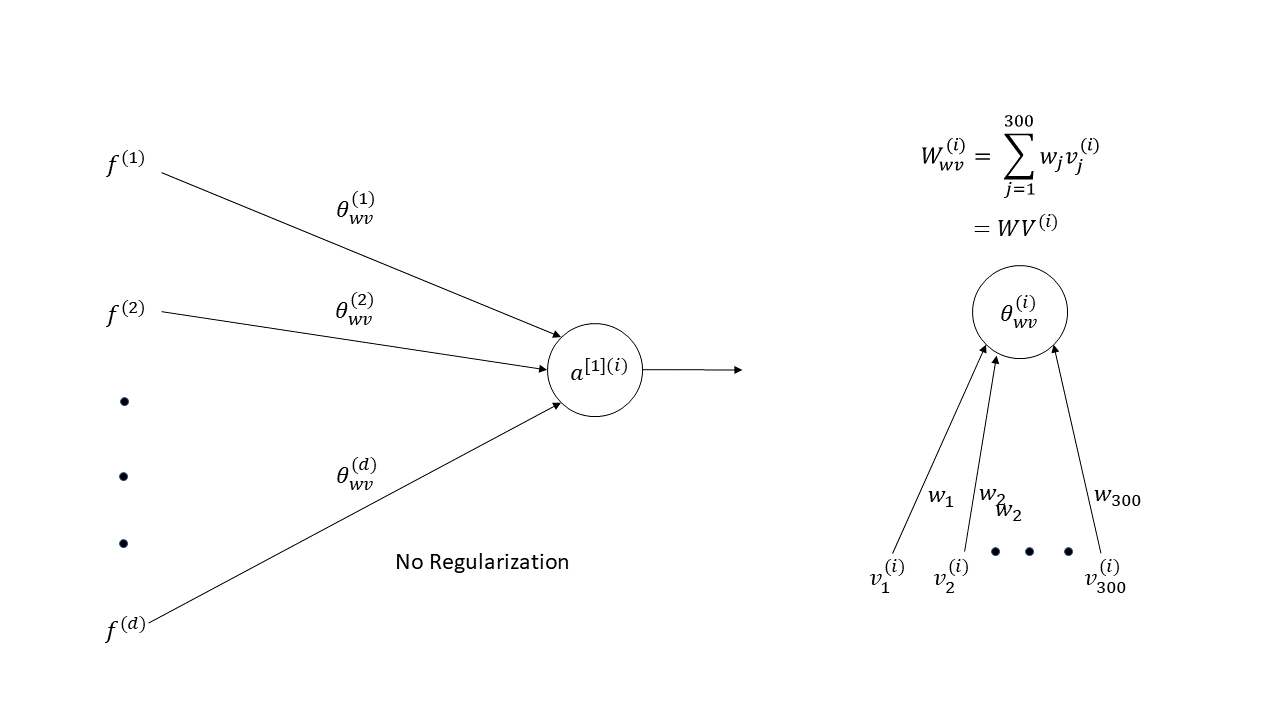
\includegraphics[width=16cm, height=8cm]{images/init-wv.png}\\
\centering
\caption{Initial word-vectors model}
\label{fig:foo}
\end{figure}

\newpage
\subsection{Vanilla logistic regression with word-vector regularization}

Our proposed method trained a model using coefficients trained from both the vanilla logistic regression model and word-vectors. In this model, instead of generating the feature weights using the word-vectors, we use the word-vectors as a regularizer that is added to the cost function. This regularizer would add a higher penalty to similar words having large differences in their corresponding feature weights. This kind of regularization should technically enforce similar words to have similar weights.

Thus, similar to logistic regression the probability the class variable $y_{j}=1, j=1,2,...m$ can be modelled as follows:

\begin{equation}
\ P(y_{j}  = 1 | x_{j}; \theta) = h_{\theta}(x_{j}) = \frac{1}{1+e^{-\theta^{T}x_{(j)}}}
\end{equation}

Using the principle of maximum likelihood estimate, we find the parameters that maximize the likelihood P(X $|$ y). Hence the log-likelihood is given as,

\begin{equation}
\ L(\theta) = \sum_{i=1}^{m}{y_{i}log(h_{\theta}(x_{i})) + (1-y_{i})log(1-h_{\theta}(x_{i}))}
\end{equation}

Maximizing the log-likelihood is similar to minimizing -L($\theta$) over all data points. The cost function for the logistic regression model comes out to be,

\begin{equation}
\ J(\theta) = -\frac{1}{m}{L(\theta)}
\end{equation}

Adding L1, L2 and word-vector regularization to this we get:

\begin{equation}
\ J(\theta) = -\frac{1}{m}{L(\theta)} + \frac{\lambda_{1}}{m}{|{\theta}|} + \frac{\lambda_{2}}{m}{|{\theta}|}^{2} + 
\frac{\lambda_{3}}{m}{(WV Reg)}
\end{equation}

where $\lambda_{1}, \lambda_{2}, \lambda_{3}$ and l1, l2 and word-vector regularization constraints.\\

\noindent Given a dataset of $n$ features, we compute the word-vector regularization as follows:

\begin{itemize}
\item Compute the cosine similarity between all feature's words-vectors. This will give us a $(n$ x $n)$ dimensional similarity matrix
\item Compute the difference between the corresponding feature weights $\theta$. This will also give us an $(n$ x $n)$ dimensional matrix that contains the difference between a feature's weight to all other weights
\item Perform a matrix multiplication between the similarity matrix and the matrix having the difference between the coefficients
\item The final result will act as a word-vector regularizer which can be added to the overall cost function regularized by a regularization parameter $\lambda_{3}$

\end{itemize}

\newpage

\begin{figure}[htbp]
\centering
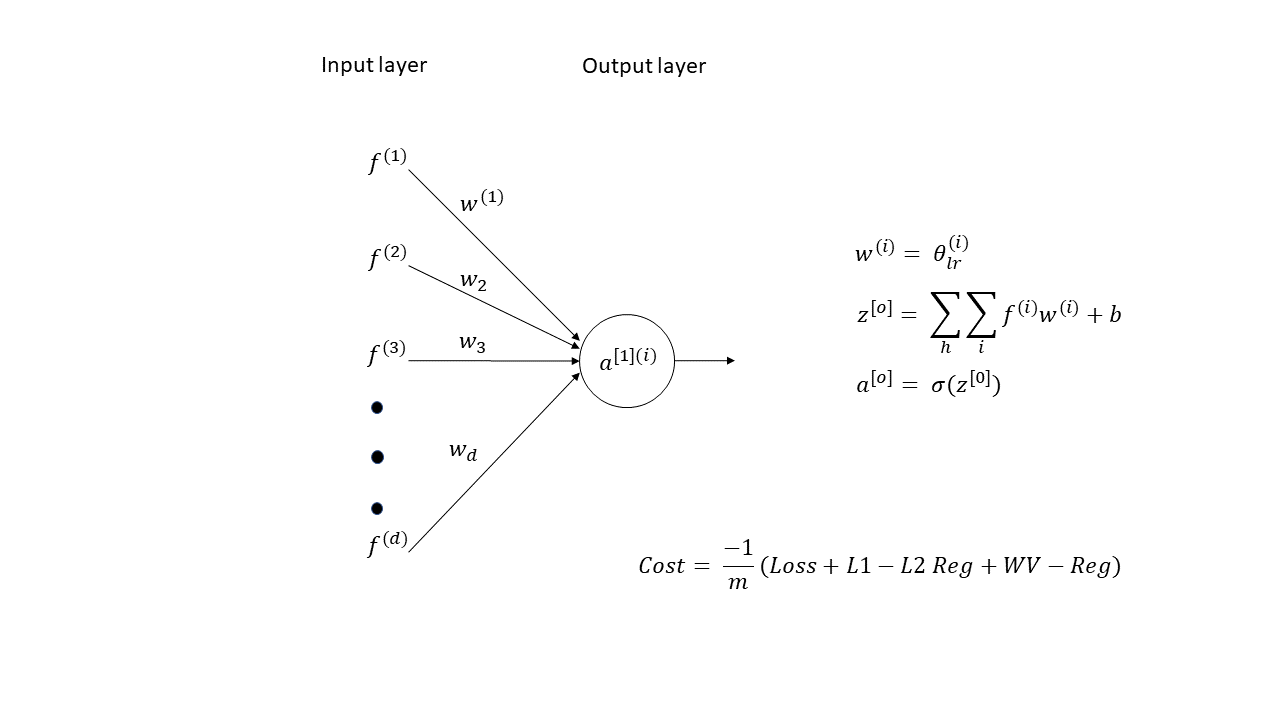
\includegraphics[width=16cm, height=10cm]{images/model3.png}\\
\centering
\caption{Logistic Regression with Word-vector regularization}
\label{fig:foo}
\end{figure}

\subsubsection{Why would it work?}

Let's say there are two words "Russia" and "Soviet" having similar word-vectors due to their reference in similar context. However the word "Russia" is present in the text more often than "Soviet" and has higher feature weight. Due to their high similarity and larger difference in weights, the word-vector model will add a higher penalty to the cost function until their corresponding weights are close to each other.

Now the claim is that the cost function would be minimized if the word-vector penalty is minimum. Now let's think about a few cases: 

\begin{itemize}
    \item \textbf{Case 1:} If two features $x_{i}$, $x_{j}$ are completely dissimilar, their cosine similarity is 0, and they don't contribute to the cost function
    \item \textbf{Case 2:} If two features are completely alike, their cosine similarity is 1. Now we have two subcases:
    \begin{itemize}
        \item \textbf{Subcase 1:} Both features have similar weights, thus the difference between their weights is 0. This would also not contribute to the cost function.
        
        \item \textbf{Subcase 2:} Both features have very different weights, thus the difference between their weights would be large. This would \textit{increase} the overall cost function. This is precisely the examples we are looking for: similar features having very different weights. So the algorithm forces them to have the same weights.
    \end{itemize}
\end{itemize}

\subsubsection{Challenges faced}

The major challenge faced while running this model is the amount of time it took to generate the weight differences matrix and computing its dot product with the similarity matrix. Since the model was trained using mini-batch gradient descent, we had to compute the word-vector regularization cost at the end of every mini-batch in order to update the weights. 

So for a medium sized dataset with 10,000 features, 100,000 records and a decent batch size of 10\% of training data, one would have to compute these matrices and get their dot product at least 10 times. And that would train the model for just a single epoch. For training a good enough model with a decent learning rate, one would need to train the model for at least 400-500 epochs. All of this only if we are training a binary classifier. If we are training a multi-class or multi-label classifier with $\sim$2000 different classes, then it would take an exponential amount of time. This puts a huge constraint on the amount of time and resources needed to train the model. For training an even larger dataset with $\sim$100,000 features, it would be even more difficult as training a single epoch itself might take a few hours.

\subsubsection{Workarounds}

In order to remediate this, we limit the features for which we want to increase the weights. Since our objective through this project was to make rare features have higher weights, we can pick the top k rarest features and look at their similarities with the rest of the features. This would reduce the similarity matrix size from $(n$ x $n)$ to $(n$ x $k)$. We can choose the top rare features based on their IDF (Inverse Document Frequency) score.

Inverse docment frequency or IDF is a numerical statistic used in information retrieval to reflect how rare a term is. It is known that certain terms, such as "is", "of", and "that" may appear a lot of times but have little importance. IDF helps in weighing down the frequent terms and finding the rare ones by computing the following:

\begin{equation}
\ IDF = log_e (\frac{Total number of documents}{Number of documents with term t in it})
\end{equation}

Once we decide on the total number of top rare features, the rest of the steps remain same as before with the only change being that we compute the cosine similarity and difference in coefficients matrix for only these top features and add the resulting value as the word-vector regularization cost.

\iffalse
\newpage
\subsubsection{Model Performance}

Below is a table showing how our model performed as compared to the pyramid and tensorflow implementation of vanilla logistic regression.

\begin{table}[htbp]
\centering
\begin{tabular}{l|c|c|c|}
Datasets    & \multicolumn{1}{l|}{\begin{tabular}[c]{@{}l@{}}Pyramid LR\\ Set Accuracy\end{tabular}} & \multicolumn{1}{l|}{\begin{tabular}[c]{@{}l@{}}Tensorflow LR\\ Set Accuracy\end{tabular}} & \multicolumn{1}{l|}{\begin{tabular}[c]{@{}l@{}}LR + WV Reg\\ Set Accuracy\end{tabular}} \\ \hline
IMDb        & 19.66                                                                                  & 18.21                                                                                     & 17.19                                                                                   \\
20Newsgroup & 55.64                                                                                  & 55.75                                                                                     & 56.32                                                                                  
\end{tabular}
\caption{\label{tab:widgets}Set-Accuracy Results.}
\end{table}

\begin{table}[htbp]
\centering
\begin{tabular}{l|c|c|c|}
Datasets    & \begin{tabular}[c]{@{}c@{}}Pyramid LR\\ Instance-F1\end{tabular} & \begin{tabular}[c]{@{}c@{}}Tensorflow LR\\ Instance-F1\end{tabular} & \begin{tabular}[c]{@{}c@{}}LR + WV Reg\\ Instance-F1\end{tabular} \\ \hline
IMDb        & 56.14                                                            & 57.87                                                               & 47.67                                                             \\
20Newsgroup & 55.64                                                            & 55.75                                                               & 55.48                                                            
\end{tabular}
\caption{\label{tab:widgets}Instance-F1 Results.}
\end{table}

Based on the above model performance, we can see that the word-vector regularization model did not perform that well as compared to the vanilla logistic regression model. This could be due to the fact that there our model was restricted by the total number of rare features we could use to regularize the model along with the added regularization constraint.

\fi
\newpage
\section{Experiments}

% \section{Baseline}

We compare our model to the vanilla logistic regression algorithm by implementing both using the TensorFlow library. Both the models can perform multi-class and multi-label classification. For multi-class, we use the softmax function to assign probabilities to each class which add up to 1. We use the sigmoid function for multi-label classification to train an independent logistic regression model for each class and accept all labels greater than a certain threshold as predictions.

We tune our model using learning rate and regularization parameter as hyper-parameters and train with different number of epochs till the loss converges. For multi-label problems, we also use prediction threshold as one of the hyper-parameters to list labels with probabilities greater than the threshold value.

\subsection{Evaluation}

To evaluate the performance of both models for multi-class problems, we use accuracy and F1 measures.

For multi-label problems, predictions for an instance is a set of labels, and therefore the prediction can be fully correct, partially-correct or fully-incorrect. Thus, to better evaluate our models we will use the following three measures: \textit{set accuracy}, which is the ratio of perfectly matched instances to the total number of instances; \textit{instance-F1}, which evaluates the performance of partially correct predictions averaged over instances; \textit{label-F1}, which evaluates the performance of partially correct predictions averaged over labels.\\

For a dataset with ground truth labels $y^{(n)}$ and predictions $\hat{y}^{(n)}$, and n instances where n = 1,2,...,N, these three measures are defined as:

\begin{alignat}{2}
set\; accuracy & = \frac{1}{N} \sum_{n=1}^{N} {I(y^{(n)} = \hat{y}^{(n)})}\\
instance \mbox{-} F1 & = \frac{1}{N} \sum_{n=1}^{N} \frac{2\sum_{l=1}^{L} {y^{(n)}_{l} \hat{y}^{(n)}_{l}}}{\sum_{l=1}^{L} {y^{(n)}_{l}} + \sum_{l=1}^{L} {\hat{y}^{(n)}_{l}}}
\hspace{6ex}
label \mbox{-} F1 & = \frac{1}{N} \sum_{n=1}^{N} \frac{2\sum_{n=1}^{N} {y^{(n)}_{l} \hat{y}^{(n)}_{l}}}{\sum_{n=1}^{N} {y^{(n)}_{l}} + \sum_{n=1}^{N} {\hat{y}^{(n)}_{l}}}
\end{alignat}

\noindent where for each instance $n$, $y^{(n)}_{l}$ = 1 if label $l$ is a given label in ground truth; \\
$\hat{y}^{(n)}_{l}$ = 1 if label $l$ is a predicted label.
\newpage
\subsection{Datasets}

\subsubsection{IMDb}

The IMDb dataset is created by Meka with movie plot text summaries labelled with genres sourced from the Internet Movie Database Interface. It is a collection of 35,000 documents partitioned across 25 different genres. The task is to assign multiple genres to a movie description.

Below is a list of the 25 different genres with individual genre counts.

\begin{table}[htbp]
\begin{tabular}{ll|ll}
Drama       & 11726 & Family    & 1564 \\
Comedy      & 7279  & Biography & 1151 \\
Romance     & 4488  & War       & 1049 \\
Thriller    & 4468  & Animation & 949  \\
Crime       & 3195  & History   & 932  \\
Action      & 3120  & Music     & 827  \\
Horror      & 2414  & Musical   & 687  \\
Adventure   & 2313  & Western   & 574  \\
Documentary & 1895  & Short     & 546  \\
Mystery     & 1775  & Sport     & 471  \\
Sci-Fi      & 1692  & Film-Noir & 257  \\
Fantasy     & 1612  & News      & 68  
\end{tabular}
\caption{\label{tab:widgets}The 24 topic categories for the IMDb dataset with the number of examples assigned to them.}
\end{table}

\subsubsection{Guardian}

The Guardian is a National British daily newspaper, known until 1959 as the Manchester Guardian. Its online edition was the fifth most widely read in the world as of October 2014, with over 42 million readers. This dataset contains articles on various topics like World news, UK news, Culture, Politics, Media, Business, Society etc.

All the data had been manually scrapped from the Guardian website with each file containing a document and its associated tags. The dataset in use contains 20 different classes and the task is to assign multiple tags to each news article.

Below is a list of the 20 different genres.

\begin{table}[htbp]
\begin{tabular}{l|l}
Blogging       & LGBT rights    \\
Christianity      & Mental health \\
Comedy     & Poetry       \\
Computing    & Premier League \\
Counter-terrorism policy      & Public finance   \\
Drugs      & Public sector cuts     \\
Financial crisis      & Research   \\
Global enonomy   & Restaurants   \\
Health policy & Retail industry     \\
Inequality     & Tax and spending      
\end{tabular}
\caption{\label{tab:widgets}The 20 topic categories for the Guardian dataset with the number of examples assigned to them.}
\end{table}

\newpage
\subsubsection{20 Newsgroups}

The 20 Newsgroups dataset is a collection of approximately 20,000 newsgroup documents, partitioned (nearly) evenly across 20 different newsgroups. It has become a popular data set for experiments in text applications of machine learning techniques, such as text classification and text clustering.

The data is organized into 20 different newsgroups, each corresponding to a different topic. Some of the newsgroups are very closely related to each other (e.g.\textbf{ comp.sys.ibm.pc.hardware / comp.sys.mac.hardware}), while others are highly unrelated (e.g \textbf{misc.forsale / soc.religion.christian}). Except for a small fraction of the articles, each document belongs to exactly one newsgroup. The task is to learn which newsgroup an article was posted to. Below is a list of 20 newsgroup partitioned according to their subject matter.\\

\begin{table}[htbp]
\begin{tabular}{|l|l|l|lllllll}
\cline{1-3}
comp.graphics            &                       &                        &  &  &  &  &  &  &  \\
comp.os.ms-windows.misc  & rec.autos             & sci.crypt              &  &  &  &  &  &  &  \\
comp.sys.ibm.pc.hardware & rec.motorcycles       & sci.electronics        &  &  &  &  &  &  &  \\
comp.sys.mac.hardware    & rec.sport.baseball    & sci.med                &  &  &  &  &  &  &  \\
comp.windows.x           & rec.sport.hockey      & sci.space              &  &  &  &  &  &  &  \\ \cline{1-3}
                         & talk.politics.misc    & talk.religion.misc     &  &  &  &  &  &  &  \\
misc.forsale             & talk.politics.guns    & alt.atheism            &  &  &  &  &  &  &  \\
                         & talk.politics.mideast & soc.religion.christian &  &  &  &  &  &  &  \\ \cline{1-3}
\end{tabular}
\caption{\label{tab:widgets}Newsgroups used in newsgroups data}
\end{table}

\newpage
\subsection{Model Performance}

Below is a table showing how our model performed as compared to the pyramid and tensorflow implementation of vanilla logistic regression.

\begin{table}[htbp]
\centering
% \resizebox{\textwidth}{!}{%
\begin{tabular}{l|c|c|c|c}
Datasets & \begin{tabular}[c]{@{}c@{}}Pyramid LR\\ Set Accuracy\end{tabular} & \begin{tabular}[c]{@{}c@{}}Tensorflow LR\\ Set Accuracy\end{tabular} & \begin{tabular}[c]{@{}c@{}}Our model\\ Set Accuracy\end{tabular}\\\hline
IMDb & 19.66 & 18.21 & 20.30\\
20Newsgroup & 55.64 & 55.75 & 58.80\\
Guardian & 59.3 & 53.46 & 59.3\\
\end{tabular}%
% }
\caption{\label{tab:widgets}Set-Accuracy Results.}
\end{table}

\begin{table}[htbp]
\centering
% \resizebox{\textwidth}{!}{%
\begin{tabular}{l|c|c|c|c}
Datasets & \begin{tabular}[c]{@{}c@{}}Pyramid LR\\ Instance-F1\end{tabular} & \begin{tabular}[c]{@{}c@{}}Tensorflow LR\\ Instance-F1\end{tabular} & \begin{tabular}[c]{@{}c@{}}Our model\\ Instance-F1\end{tabular}\\\hline
IMDb & 56.14 & 57.87 & 58.52\\
20Newsgroup & 55.64 & 55.75 & 58.80\\
Guardian & 65.13 & 65.61 & 69.41\\
\end{tabular}%
% }
\caption{\label{tab:widgets}Instance-F1 Results.}
\end{table}

\noindent We also run a validation experiment with artificially modified dataset 20newsgroup to mimic sparse representation: we found the most similar words in the train set with cosine similarity greater than 0.3 and make the feature values of all but one of the words equal to zero. We then compared the performance of our model with logistic regression before and after zeroing feature values of similar words. The below results show that our model was able to get a good test accuracy after the imposed sparsity.\\


\begin{tabular}{l|c|c}
\hline
					& Logistic Regression 	& Our model \\
Before zeroing features		& 82.6			& 84.01 \\
After zeroing features		& 75.67			& 83.54\\
\hline
\end{tabular}
\newpage
\section{Analysis}
Upon comparing both models, we noticed that the performance of the word-vector models improved due to the additional word-vector weights.

To verify this, we took the top features for each model and printed the following:

\begin{itemize}
\item top similar words for each feature calculated based on the cosine similarity of the word-vectors

\item cosine similarity of the similar word

\item feature weight of the similar word

\item idf score of the similar word
\end{itemize}

The idf scores were computed to measure the rarity of the words. We noticed that the rare features which were similar to the important features now had similar weights. The below section shows such examples:

\subsection{Examples of rare-similar words now having similar weights}

In this section we show a few examples where the word-vector model is able to generate similar weights for similar words, even if some of these words are rare. The rarity of the word can be determined by their corresponding Idf score. Due to the rarity of the words, the vanilla logistic regression model did not have enough information to determine the influence of these rare words and assigned them very small weights. However the word-vector models were able to assign comparatively higher weights due to their similarity feature. \\

In the below example, we can see that \textbf{marijuana} and \textbf{narcotics} are rare features based on their higher Idf scores. Inspite of that, due to their similarity with the \textbf{drug}, they have substantially higher word-vector weights. Comparatively these rare words have very small weights when trained through vanilla logistic regression model. Thus, after using the word-vector model, when these rare words do appear in the test set, they now have a higher chance of getting classified under the class \textbf{Drug}.

\begin{table}[htbp]
\begin{tabular}{llllll}
\multicolumn{2}{l|}{\textbf{Class: Drug}}                                  & \multicolumn{1}{l|}{\textbf{\begin{tabular}[c]{@{}l@{}}vanilla\\ weights\end{tabular}}} & \multicolumn{1}{l|}{\textbf{Similarity}} & \multicolumn{1}{l|}{\textbf{Idf-score}} & \textbf{\begin{tabular}[c]{@{}l@{}}wv\\ weights\end{tabular}} \\ \hline
\multicolumn{1}{l|}{\textbf{Top-feature}} & \multicolumn{1}{l|}{cannabis}  & \multicolumn{1}{l|}{0.388}                                                              & \multicolumn{1}{l|}{1}                   & \multicolumn{1}{l|}{5.5}                & 0.159                                                         \\ \hline
\multicolumn{1}{l|}{\textbf{Top similar}} & \multicolumn{1}{l|}{marijuana} & \multicolumn{1}{l|}{0.012}                                                              & \multicolumn{1}{l|}{0.764}               & \multicolumn{1}{l|}{6}                  & 0.126                                                         \\
\multicolumn{1}{l|}{\textbf{features}}    & \multicolumn{1}{l|}{heroin}    & \multicolumn{1}{l|}{0.097}                                                              & \multicolumn{1}{l|}{0.694}               & \multicolumn{1}{l|}{4.86}               & 0.129                                                         \\
\multicolumn{1}{l|}{}                     & \multicolumn{1}{l|}{narcotics} & \multicolumn{1}{l|}{-2e-5}                                                              & \multicolumn{1}{l|}{0.557}               & \multicolumn{1}{l|}{6.19}               & 0.06                                                          \\
                                          &                                &                                                                                         &                                          &                                         &                                                              
\end{tabular}
\caption{\label{tab:widgets}Top feature weights comparison for Drugs}
\end{table}

\newpage

Here is an example which displays the vanilla and word-vector model weights for \textbf{chinese}, \textbf{shanghai} and \textbf{taiwan} which are some of the words used in similar context to \textbf{beijing}. Since \textbf{chinese} is not a rare word, we can see that its vanilla logistic regression model weight is quite high as compared to the word-vector model weight. However, when it comes across rarer words like \textbf{shanghai} and \textbf{taiwan}, its corresponding vanilla weights have dropped significantly, whereas the word-vector model weights are comparatively higher and closer to their corresponding word-vector weight of \textbf{beijing}.

\begin{table}[htbp]
\begin{tabular}{llllll}
\multicolumn{2}{l|}{\textbf{Class: China}}                                & \multicolumn{1}{l|}{\textbf{\begin{tabular}[c]{@{}l@{}}vanilla\\ weights\end{tabular}}} & \multicolumn{1}{l|}{\textbf{Similarity}} & \multicolumn{1}{l|}{\textbf{Idf-score}} & \textbf{\begin{tabular}[c]{@{}l@{}}wv\\ weights\end{tabular}} \\ \hline
\multicolumn{1}{l|}{\textbf{Top-feature}} & \multicolumn{1}{l|}{beijing}  & \multicolumn{1}{l|}{0.252}                                                              & \multicolumn{1}{l|}{1}                   & \multicolumn{1}{l|}{4.01}               & 0.215                                                         \\ \hline
\multicolumn{1}{l|}{\textbf{Top similar}} & \multicolumn{1}{l|}{chinese}  & \multicolumn{1}{l|}{0.376}                                                              & \multicolumn{1}{l|}{0.696}               & \multicolumn{1}{l|}{3.23}               & 0.166                                                         \\
\multicolumn{1}{l|}{\textbf{features}}    & \multicolumn{1}{l|}{shanghai} & \multicolumn{1}{l|}{0.075}                                                              & \multicolumn{1}{l|}{0.656}               & \multicolumn{1}{l|}{5.17}               & 0.10                                                          \\
\multicolumn{1}{l|}{}                     & \multicolumn{1}{l|}{taiwan}   & \multicolumn{1}{l|}{3e-5}                                                               & \multicolumn{1}{l|}{0.607}               & \multicolumn{1}{l|}{5.53}               & 0.073                                                         \\
                                          &                               &                                                                                         &                                          &                                         &                                                              
\end{tabular}
\caption{\label{tab:widgets}Top feature weights comparison for China}
\end{table}

Below is a similar example where \textbf{ranch} is a top feature for the class \textbf{Western}. Again we can see that the weights of rare-words \textbf{cattle}, \textbf{farm} and \textbf{sheep} have been boosted due to the word-vector model.

\begin{table}[htbp]
\begin{tabular}{llllll}
\multicolumn{2}{l|}{\textbf{Class: Western}}                             & \multicolumn{1}{l|}{\textbf{\begin{tabular}[c]{@{}l@{}}vanilla\\ weights\end{tabular}}} & \multicolumn{1}{l|}{\textbf{Similarity}} & \multicolumn{1}{l|}{\textbf{Idf-score}} & \textbf{\begin{tabular}[c]{@{}l@{}}wv\\ weights\end{tabular}} \\ \hline
\multicolumn{1}{l|}{\textbf{Top-feature}} & \multicolumn{1}{l|}{ranch}  & \multicolumn{1}{l|}{0.103}                                                              & \multicolumn{1}{l|}{1}                   & \multicolumn{1}{l|}{5.29}               & 1.216                                                         \\ \hline
\multicolumn{1}{l|}{\textbf{Top similar}} & \multicolumn{1}{l|}{cattle} & \multicolumn{1}{l|}{0.050}                                                              & \multicolumn{1}{l|}{0.716}               & \multicolumn{1}{l|}{5.55}               & 0.878                                                         \\
\multicolumn{1}{l|}{\textbf{features}}    & \multicolumn{1}{l|}{farm}   & \multicolumn{1}{l|}{-4e-5}                                                               & \multicolumn{1}{l|}{0.705}               & \multicolumn{1}{l|}{4.24}               & 0.486                                                         \\
\multicolumn{1}{l|}{}                     & \multicolumn{1}{l|}{sheep}  & \multicolumn{1}{l|}{-3e-5}                                                               & \multicolumn{1}{l|}{0.591}               & \multicolumn{1}{l|}{6.03}               & 0.314                                                         \\
                                          &                             &                                                                                         &                                          &                                         &                                                              
\end{tabular}
\caption{\label{tab:widgets}Top feature weights comparison for West}
\end{table}

The above examples do help in proving that our model was successfully able to use word-vectors as a regularizer to assign similar weights to similar words even if those similar words happen to be rare.

\newpage
\subsection{Scenarios when word-vector model doesn't work}

\begin{table}[htbp]
\begin{tabular}{llllll}
\multicolumn{2}{l|}{\textbf{Class: Western}}                           & \multicolumn{1}{l|}{\textbf{\begin{tabular}[c]{@{}l@{}}vanilla\\ weights\end{tabular}}} & \multicolumn{1}{l|}{\textbf{Similarity}} & \multicolumn{1}{l|}{\textbf{Idf-score}} & \textbf{\begin{tabular}[c]{@{}l@{}}wv\\ weights\end{tabular}} \\ \hline
\multicolumn{1}{l|}{\textbf{Top-feature}} & \multicolumn{1}{l|}{west}  & \multicolumn{1}{l|}{0.224}                                                              & \multicolumn{1}{l|}{1}                   & \multicolumn{1}{l|}{3.95}               & 0.981                                                         \\ \hline
\multicolumn{1}{l|}{\textbf{Top similar}} & \multicolumn{1}{l|}{north} & \multicolumn{1}{l|}{-4e-5}                                                              & \multicolumn{1}{l|}{0.823}               & \multicolumn{1}{l|}{4.06}               & 0.38                                                          \\
\multicolumn{1}{l|}{\textbf{features}}    & \multicolumn{1}{l|}{east}  & \multicolumn{1}{l|}{-3e-5}                                                              & \multicolumn{1}{l|}{0.822}               & \multicolumn{1}{l|}{4.26}               & 0.297                                                         \\
\multicolumn{1}{l|}{}                     & \multicolumn{1}{l|}{south} & \multicolumn{1}{l|}{5e-5}                                                               & \multicolumn{1}{l|}{0.821}               & \multicolumn{1}{l|}{3.72}               & 0.232                                                         \\
                                          &                            &                                                                                         &                                          &                                         &                                                              
\end{tabular}
\end{table}

\subsection{Scenarios when word-vector model works because of word-vector coefficients not because of similarity}

\begin{table}[htbp]
\begin{tabular}{llllll}
\multicolumn{2}{l|}{\textbf{Class: Brazil}}                                 & \multicolumn{1}{l|}{\textbf{\begin{tabular}[c]{@{}l@{}}vanilla\\ weights\end{tabular}}} & \multicolumn{1}{l|}{\textbf{Similarity}} & \multicolumn{1}{l|}{\textbf{Idf-score}} & \textbf{\begin{tabular}[c]{@{}l@{}}wv\\ weights\end{tabular}} \\ \hline
\multicolumn{1}{l|}{\textbf{Top-feature}} & \multicolumn{1}{l|}{amazon}     & \multicolumn{1}{l|}{0.086}                                                              & \multicolumn{1}{l|}{1}                   & \multicolumn{1}{l|}{4.3}                & 0.146                                                         \\ \hline
\multicolumn{1}{l|}{\textbf{Top similar}} & \multicolumn{1}{l|}{kindle}     & \multicolumn{1}{l|}{-4e-5}                                                              & \multicolumn{1}{l|}{0.699}               & \multicolumn{1}{l|}{5.96}               & 0.037                                                         \\
\multicolumn{1}{l|}{\textbf{features}}    & \multicolumn{1}{l|}{ebooks}     & \multicolumn{1}{l|}{-1e-5}                                                              & \multicolumn{1}{l|}{0.655}               & \multicolumn{1}{l|}{6.51}               & 0.004                                                         \\
\multicolumn{1}{l|}{}                     & \multicolumn{1}{l|}{rainforest} & \multicolumn{1}{l|}{1e-5}                                                               & \multicolumn{1}{l|}{0.521}               & \multicolumn{1}{l|}{5.32}               & 0.13                                                          \\
                                          &                                 &                                                                                         &                                          &                                         &                                                              
\end{tabular}
\end{table}

\begin{table}[htbp]
\begin{tabular}{llllll}
\multicolumn{2}{l|}{\textbf{Class: Crime}}                                   & \multicolumn{1}{l|}{\textbf{\begin{tabular}[c]{@{}l@{}}vanilla\\ weights\end{tabular}}} & \multicolumn{1}{l|}{\textbf{Similarity}} & \multicolumn{1}{l|}{\textbf{Idf-score}} & \textbf{\begin{tabular}[c]{@{}l@{}}wv\\ weights\end{tabular}} \\ \hline
\multicolumn{1}{l|}{\textbf{Top-feature}} & \multicolumn{1}{l|}{examination} & \multicolumn{1}{l|}{1.5}                                                                & \multicolumn{1}{l|}{1}                   & \multicolumn{1}{l|}{5.63}               & 0.245                                                         \\ \hline
\multicolumn{1}{l|}{\textbf{Top similar}} & \multicolumn{1}{l|}{tests}       & \multicolumn{1}{l|}{1e-4}                                                               & \multicolumn{1}{l|}{0.698}               & \multicolumn{1}{l|}{5.53}               & 0.003                                                         \\
\multicolumn{1}{l|}{\textbf{features}}    & \multicolumn{1}{l|}{exam}        & \multicolumn{1}{l|}{1e-5}                                                               & \multicolumn{1}{l|}{0.646}               & \multicolumn{1}{l|}{6.55}               & 0.010                                                         \\
\multicolumn{1}{l|}{}                     & \multicolumn{1}{l|}{analysis}    & \multicolumn{1}{l|}{0.496}                                                              & \multicolumn{1}{l|}{0.642}               & \multicolumn{1}{l|}{6.93}               & 0.21                                                          \\
                                          &                                  &                                                                                         &                                          &                                         &                                                              
\end{tabular}
\end{table}
\newpage
\newpage
\section{Training neural network models with single hidden layer}

So far we've only trained our model through a simple perceptron which includes one input layer and one output layer. The output layer was a single node which received its input from the previous layer, and this input was a weighted sum of the weights at each of the input nodes multiplied by the input values. This weighted sum was passed to a sigmoid activation function. We then computed the loss and updated the weights through back propagation.

In this chapter, we will create a neural network model with one input layer, one hidden layer and one output layer. The architecture of the neural network model will look as below:

\begin{figure}[htbp]
\centering
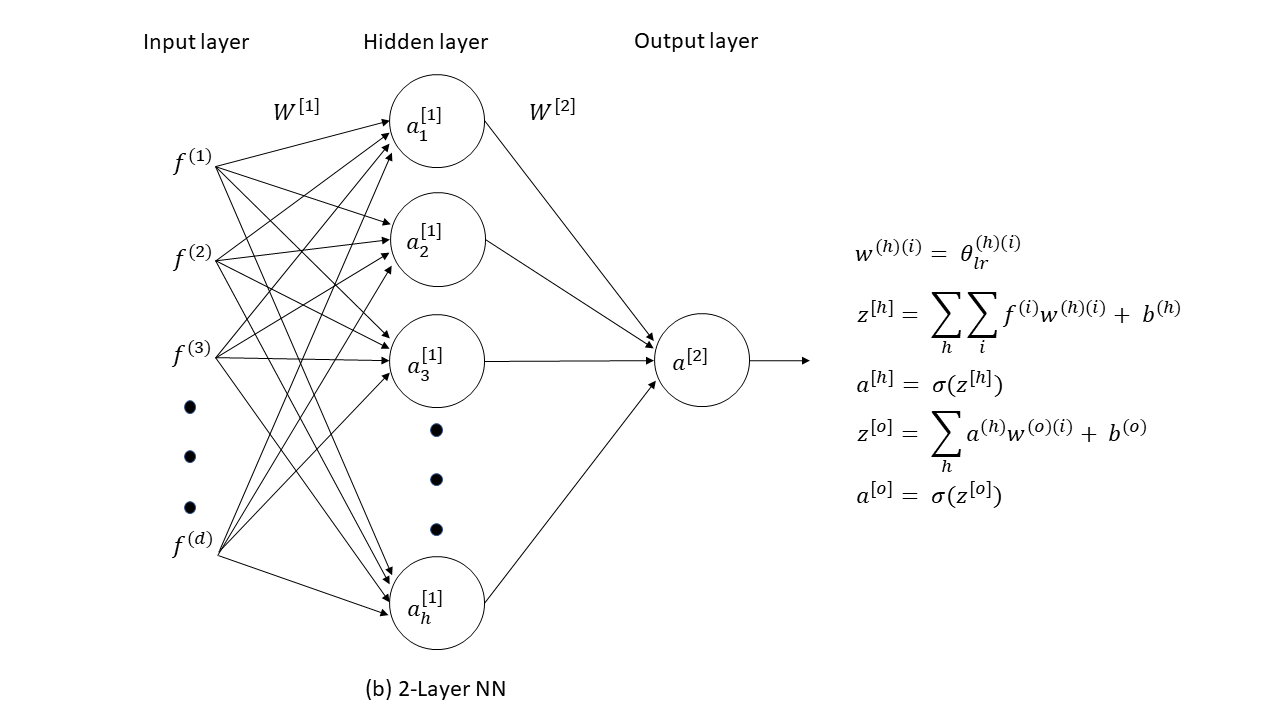
\includegraphics[width=16cm, height=10cm]{images/nn1.png}\\
\centering
\caption{Neural network model - without using word-vectors}
\label{fig:foo}
\end{figure}

In the figure above, we have a neural network with one input layer having d features, one hidden layer and one output layer. For the case of simplicity we assume we are trying to solve a binary classification problem, where there can be only two possible outputs. In reality, for multi-class classification problems, the output layer will contain multiple nodes equivalent to the total number of classes. This neural network is also capable of finding non-linear boundaries.

No matter how many nodes and hidden layers are there in a neural network, the basic working principle remains the same. We compute what the hypothesis outputs given an input through the forward propagation stage and through back propagation find the best weights that minimize the cost function.

We will build two separate models, one that uses the word-vector weights in the input layer and the one that doesn't. We then compare both model performances to see whether using the word-vector weights has improved the model performance or not.

\subsection{Neural Network model without word-vectors}

The neural network model without word-vectors is similar to using a logistic regression model with one extra hidden layer. We can look at how to perform feed-forward and back-propagation steps for this neural network.\\

\noindent \textbf{Feed Forward:}\\

We know that the input for node $j$ in layer $l$ is the weighted sum of the activation outputs from the previous layer $l-1$. So, the input for a given hidden node $h$ is expressed as:

\begin{equation}
z^{[h]} = \sum_{h}\sum_{i} f^{(i)}w^{(h)(i)} + b^{(h)}
\end{equation}

where, $f^{(i)}$ is the feature value of feature $i$

$\quad\qquad\ w^{(h)(i)} = \theta_{lr}^{(h)(i)}$ is the weight of hidden layer $h$ for input feature $i$

$\quad\qquad\ b$ is the bias added to the network\\

To that input node, we apply the activation function which in our case would be a sigmoid activation function given as:

\begin{equation}
a^{[h]} = \sigma(z^{[h]})
\end{equation}

where, $\sigma$ is the sigmoid activation function given as $\frac{1}{1+e^{-z^[h]}}$\\

This activation function output for each hidden layer is then passed as part of the input for the node in the output layer to which a sigmoid function is applied for binary classification.

\begin{equation}
z^{[o]} = \sum_{h} a^{(h)}w^{(o)(i)} + b^{(o)}
\end{equation}

\begin{equation}
a^{[o]} = \sigma(z^{[o]})
\end{equation}

\noindent \textbf{Back Propagation:}\\

Once we reach the output layer, we obtain the resulting output from the model for the given input. We then compute the loss which is the difference between the predicted and actual output.

\begin{equation}
\frac{\partial cost}{\partial a^{[o]}} = a^{[o]}-y
\end{equation}

Our objective is to minimize the loss by updating the weights of the output layer and the hidden layer. The loss of an individual node is actually a function of the activation output for that node, which itself is a function of the input to that node, and that input is a function of the weights that connect all the nodes in the previous layer to this node. Thus, the loss function is actually a composition of all of these functions.

To differentiate a composition of functions, we use the chain rule. We're needing to calculate derivatives that depend on components later in the network first and then use these derivatives in our calculations for the gradient of the loss wrt the weights that come earlier in the network. So we achieve this by repeatedly applying the chain rule in the backwards fashion.\\

\noindent Using the chain rule, the change in cost wrt weights $w^{[o]}$ and $w^{[h]}$ is given as:

\begin{equation}
\frac{\partial cost}{\partial w^{[o]}} = \frac{\partial cost}{\partial a^{[o]}} * \frac{\partial a^{[o]}}{\partial z^{[o]}} * \frac{\partial z^{[o]}}{\partial w^{[o]}}
\end{equation}

\begin{equation}
\frac{\partial cost}{\partial w^{[h]}} = \frac{\partial cost}{\partial a^{[h]}} * \frac{\partial a^{[h]}}{\partial z^{[h]}} * \frac{\partial z^{[h]}}{\partial w^{[h]}}
\end{equation}

where, $\frac{\partial a^{[o]}}{\partial z^{[o]}} =  \sigma^{'}(z^{[o]})$\\

$\quad\qquad\ \frac{\partial z^{[h]}}{\partial w^{[h]}} = a^{[h]}$ \\

The partial derivatives of the hidden layer can also be computed in a similar way. We can then update the weights as:

\begin{equation}
w^{[o]} = w^{[o]} - lr * \frac{\partial cost}{\partial w^{[o]}}
\end{equation}

\begin{equation}
w^{[h]} = w^{[h]} - lr * \frac{\partial cost}{\partial w^{[h]}}
\end{equation}

where, lr is the learning-rate of the network\\

This completes one training cycle. We need to repeat this cycle several times until convergence.

\newpage
\subsection{Neural Network model with word-vectors}

The neural network model with word-vectors is trained in a similar way as the previous model with one difference that the weights of the hidden layer would be learnt similar the earlier proposed model in Chapter 3, i.e, the weights would be a sum of both logistic regressin and word-vector weights. Thus the hidden layer weights would be given as:

\begin{equation}
w^{(h)(i)} = \theta_{lr}^{(h)(i)} + \theta_{wv}^{(h)(i)}
\end{equation}

\begin{figure}[htbp]
\centering
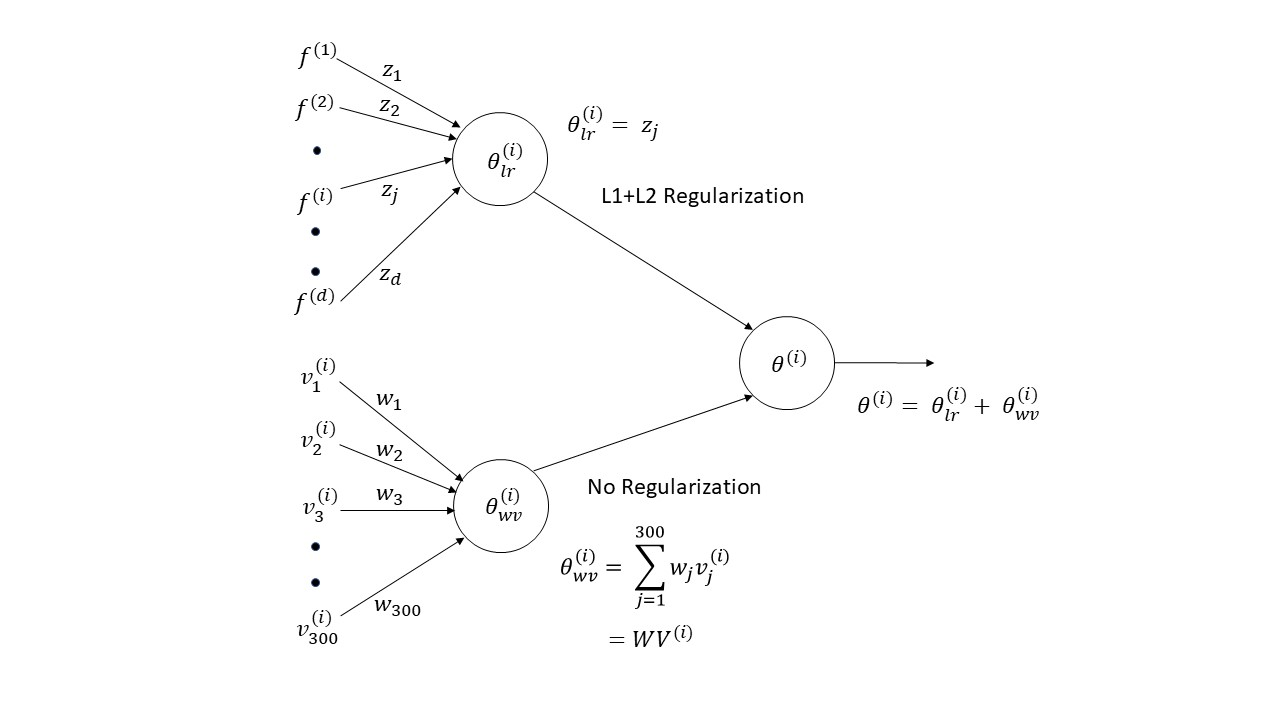
\includegraphics[width=16cm, height=10cm]{images/Fig3.jpg}\\
\centering
\caption{Network diagram to learn $w^{(h)(i)}$ from word$_{i}$ representation f(v$^{(i)}$)}
\label{fig:foo}
\end{figure}

\begin{figure}[htbp]
\centering
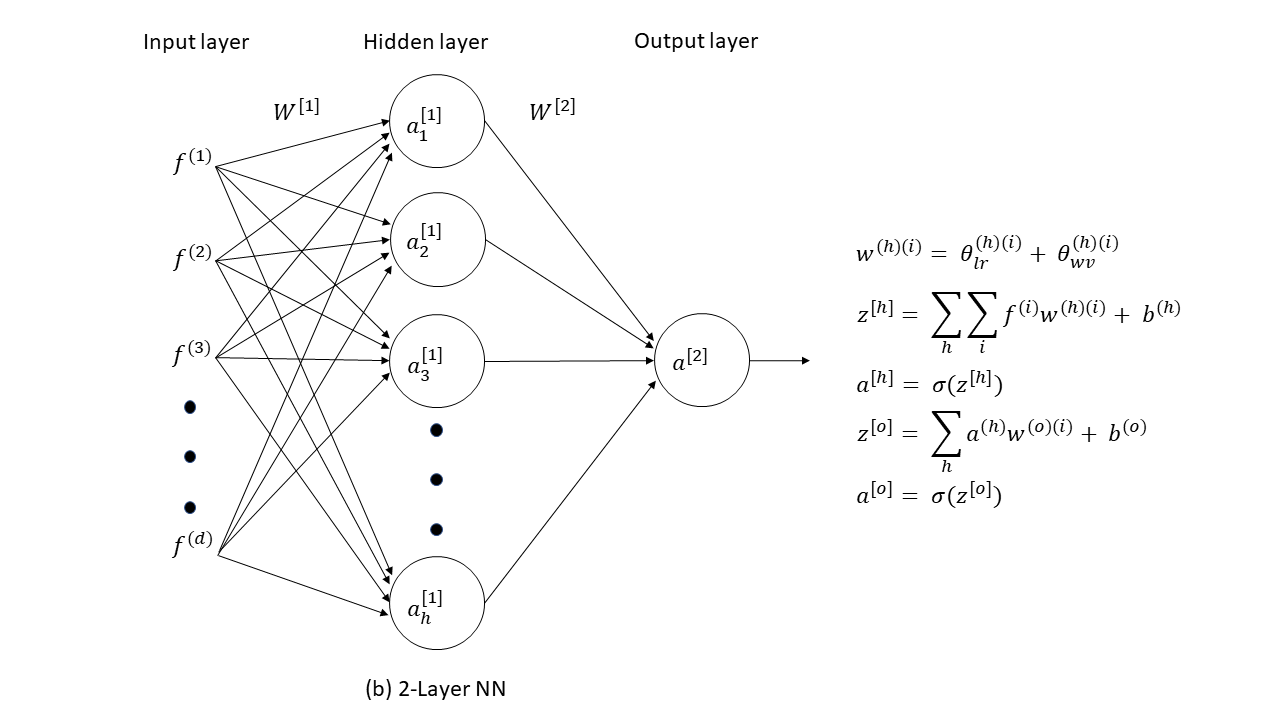
\includegraphics[width=16cm, height=10cm]{images/nn2.png}\\
\centering
\caption{Neural network model - with word-vectors}
\label{fig:foo}
\end{figure}

Computing the weights through forward propagation and updating the weights through back propagation would be similar to the previous model.

\newpage
\subsection{Model Performance}

Below is a table showing how a neural network model with one hidden layer performed with and without using features generated by word-vectors.

\begin{table}[htbp]
\centering
\begin{tabular}{llllll}
\multicolumn{1}{l|}{Datasets}    & \multicolumn{1}{c|}{\begin{tabular}[c]{@{}c@{}}1 layer NN\\ Set Accuracy\end{tabular}} & \multicolumn{1}{c|}{\begin{tabular}[c]{@{}c@{}}1 layer NN with wv\\ Set Accuracy\end{tabular}} &  &  &  \\ \cline{1-3}
\multicolumn{1}{l|}{IMDb}        & \multicolumn{1}{c|}{13.2}                                                              & \multicolumn{1}{c|}{19.63}                                                                     &  &  &  \\
\multicolumn{1}{l|}{20NewsGroup} & \multicolumn{1}{c|}{49.23}                                                                  & \multicolumn{1}{c|}{59.89}                                                                     &  &  &  \\
\end{tabular}
\caption{\label{tab:widgets}Set-Accuracy Results}
\end{table}


\begin{table}[htbp]
\centering
\begin{tabular}{llllll}
\multicolumn{1}{l|}{Datasets}    & \multicolumn{1}{c|}{\begin{tabular}[c]{@{}c@{}}1 layer NN\\ Instance F1\end{tabular}} & \multicolumn{1}{c|}{\begin{tabular}[c]{@{}c@{}}1 layer NN with wv\\ Instance F1\end{tabular}} &  &  &  \\ \cline{1-3}
\multicolumn{1}{l|}{IMDb}        & \multicolumn{1}{c|}{51.13}                                                            & \multicolumn{1}{c|}{60.21}                                                                    &  &  &  \\
\multicolumn{1}{l|}{20NewsGroup} & \multicolumn{1}{c|}{48.71}                                                                 & \multicolumn{1}{c|}{58.97}                                                                    &  &  &  \\
\end{tabular}
\caption{\label{tab:widgets}Instance F1 Results}
\end{table}

We can see that for both the datasets, the neural network model using features generated by word-vectors is the better performing model. In fact this model even outperforms all other previously tested models.

\newpage
\bibliographystyle{unsrt}
\bibliography{References}

%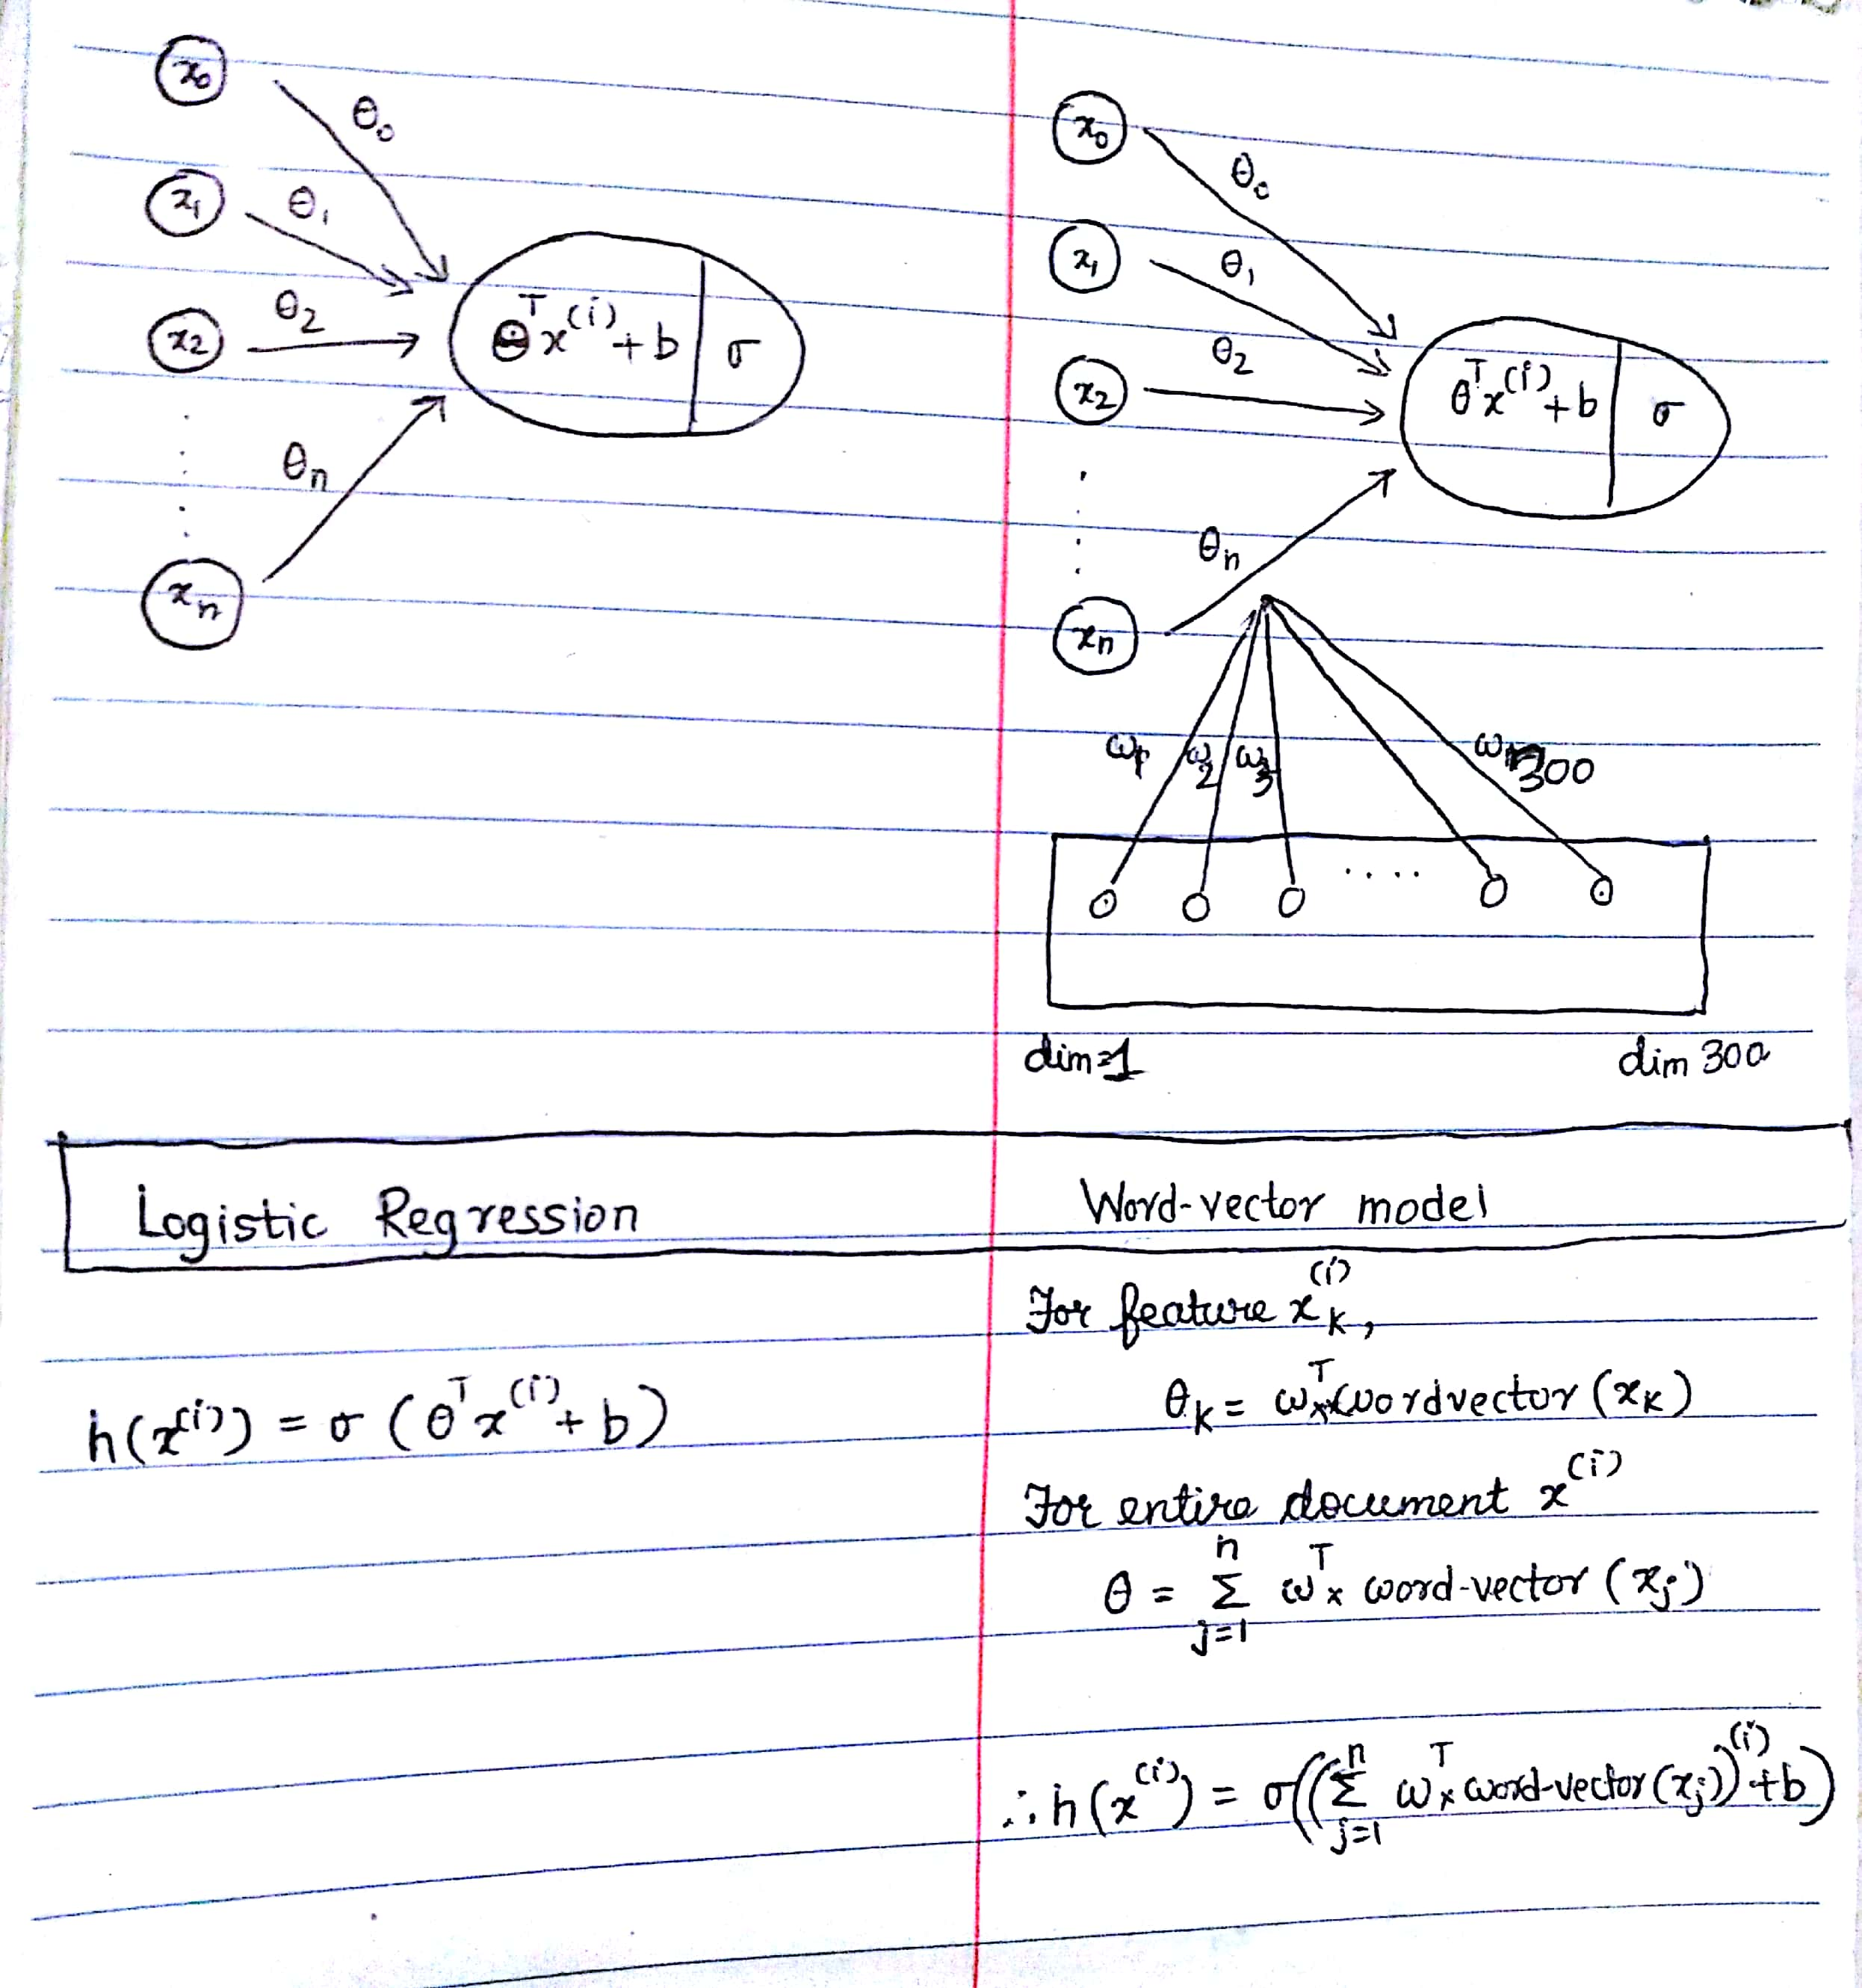
\includegraphics[width=16cm, height=10cm]{wordvec.jpg}\\[1cm]
%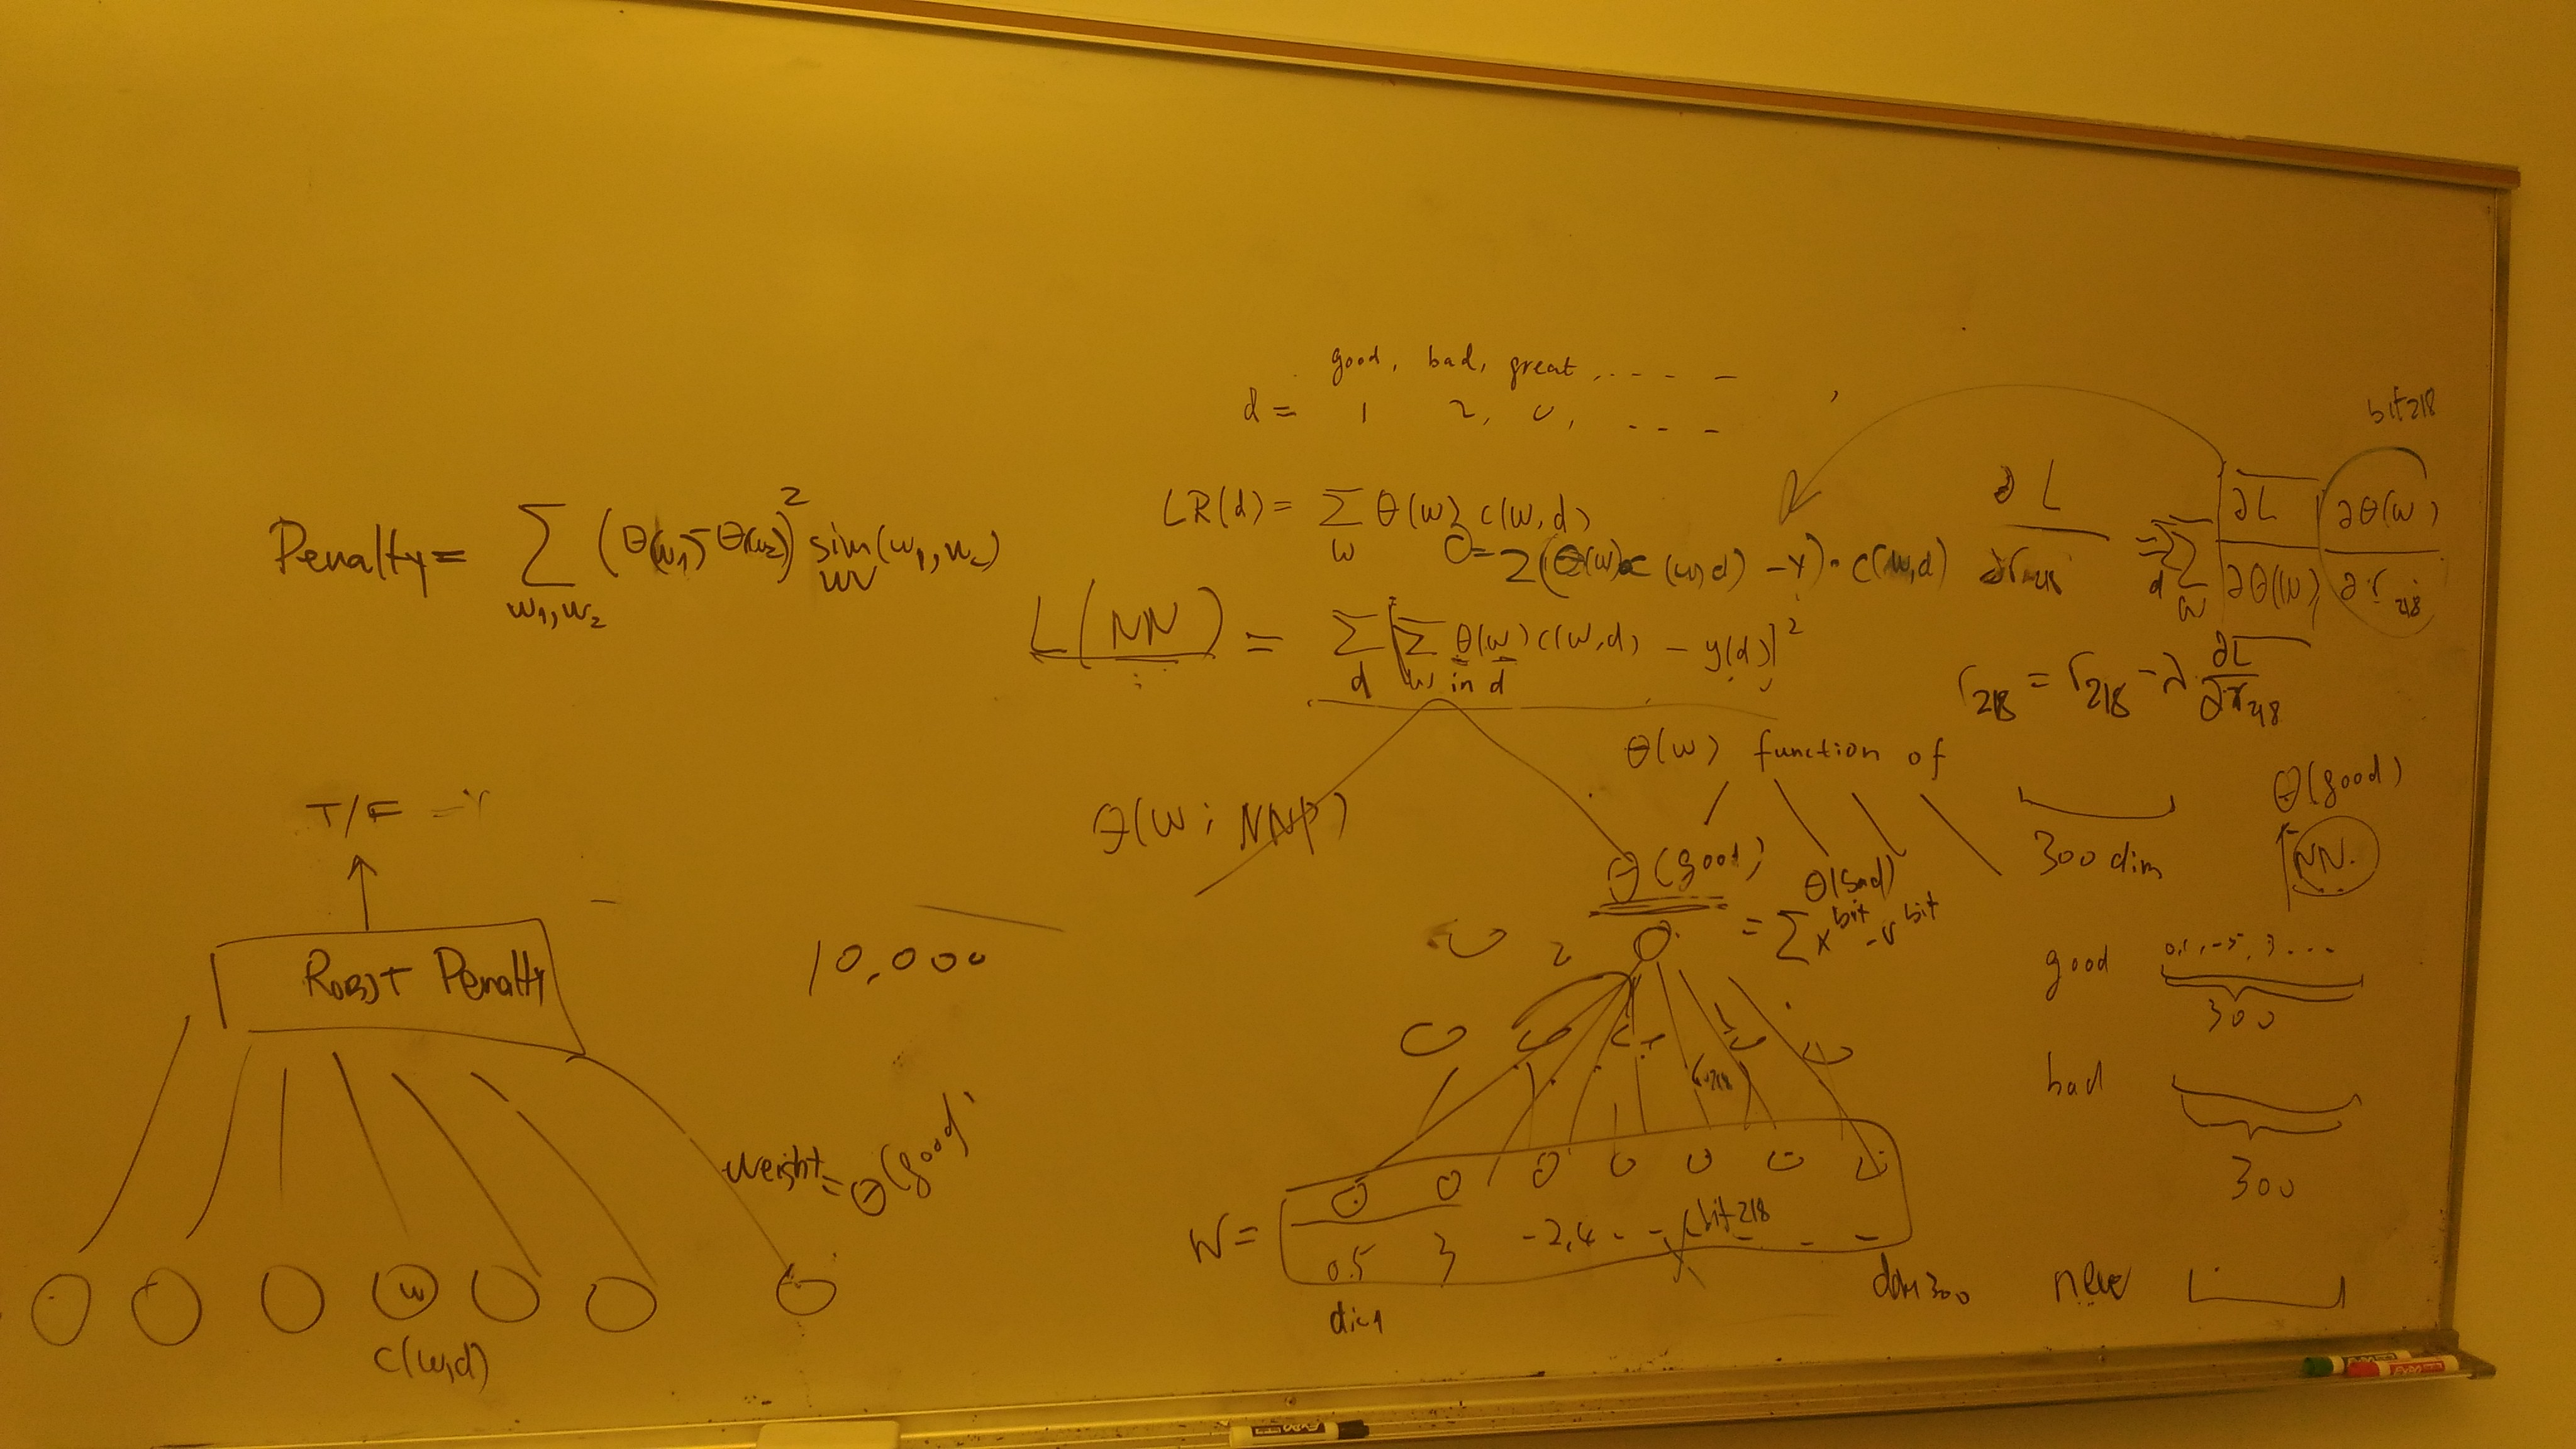
\includegraphics[width=16cm, height=10cm]{cheng.jpg}\\[1cm]

\end{document}